%\documentclass[12pt,a4paper,twoside]{book}
% @PETER
\documentclass[12pt,a4paper,twoside,parskip=full]{book}

%include the configuration file for layout
%Have a look in this file it has some useful commands defined
\usepackage{setspace}
\usepackage{geometry}
\usepackage[toc,page]{appendix}
\usepackage{lipsum}
\usepackage[export]{adjustbox}
\usepackage[T1]{fontenc}
\usepackage{textcomp}
\usepackage{epsfig,graphics}
\usepackage{graphicx}
\usepackage{titlesec}

% @PETER
\usepackage{amsthm}
\usepackage{amssymb}

% For psudocode
\usepackage{algorithm}
\usepackage[noend]{algpseudocode}

\usepackage{parskip}

% For making definitions, lemma, theorems, etc.
\newtheorem{defn}{Definition}
\newtheorem{lem}{Lemma}
\newtheorem{thm}{Theorem}

%%%%%%%%%%%%%%%%%%%%%%%%%%%%%%%%%%%%%%%%%%%%%%%%%%%%%%%%%%%%%%%%%%%%%%%%%%%%%%
% Details of your dissertation
%%%%%%%%%%%%%%%%%%%%%%%%%%%%%%%%%%%%%%%%%%%%%%%%%%%%%%%%%%%%%%%%%%%%%%%%%%%%%%
\newcommand{\projectTitle}{<Full title of Project>}
\newcommand{\fullname}{<Full Name of Author>}
\newcommand{\degreeTitle}{<Name of Degree>}
\newcommand{\session}{<Session>}

%%%%%%%%%%%%%%%%%%%%%%%%%%%%%%%%%%%%%%%%%%%%%%%%%%%%%%%%%%%%%%%%%%%%%%%%%%%%%%
% Change the geometry of the page to have a 25 mm binding edge
%%%%%%%%%%%%%%%%%%%%%%%%%%%%%%%%%%%%%%%%%%%%%%%%%%%%%%%%%%%%%%%%%%%%%%%%%%%%%%
 \geometry{
 a4paper,
 total={210mm,297mm},
 left=25mm,
 right=25mm,
 top=25mm,
 bottom=20mm,
 }
 
%%%%%%%%%%%%%%%%%%%%%%%%%%%%%%%%%%%%%%%%%%%%%%%%%%%%%%%%%%%%%%%%%%%%%%%%%%%%%%
% Commands to set the line spacing
%%%%%%%%%%%%%%%%%%%%%%%%%%%%%%%%%%%%%%%%%%%%%%%%%%%%%%%%%%%%%%%%%%%%%%%%%%%%%%
 %\singlespacing
 \onehalfspacing
 %\doublespacing
 
%%%%%%%%%%%%%%%%%%%%%%%%%%%%%%%%%%%%%%%%%%%%%%%%%%%%%%%%%%%%%%%%%%%%%%%%%%%%%%
% Spacing for the chapter header
%%%%%%%%%%%%%%%%%%%%%%%%%%%%%%%%%%%%%%%%%%%%%%%%%%%%%%%%%%%%%%%%%%%%%%%%%%%%%%
 \titleformat{\chapter}[display]
    {\normalfont\Huge\bfseries}{\vspace*{-1\baselineskip}\chaptertitlename\ \thechapter}{15pt}{\huge}
\titlespacing*{\chapter}{0pt}{0pt}{15pt}

\renewcommand\bibname{References}

%%%%%%%%%%%%%%%%%%%%%%%%%%%%%%%%%%%%%%%%%%%%%%%%%%%%%%%%%%%%%%%%%%%%%%%%%%%%%%
% Some shortcuts that maybe useful
%%%%%%%%%%%%%%%%%%%%%%%%%%%%%%%%%%%%%%%%%%%%%%%%%%%%%%%%%%%%%%%%%%%%%%%%%%%%%%
\DeclareTextCommandDefault{\textcopyright}{\textcircled{c}}
 
%%%%%%%%%%%%%%%%%%%%%%%%%%%%%%%%%%%%%%%%%%%%%%%%%%%%%%%%%%%%%%%%%%%%%%%%%%%%%%
% Bibliography style: choose one and make sure you have the relevant .bst file
%%%%%%%%%%%%%%%%%%%%%%%%%%%%%%%%%%%%%%%%%%%%%%%%%%%%%%%%%%%%%%%%%%%%%%%%%%%%%%
\bibliographystyle{abbrv}


%%%%%%%%%%%%%%%%%%%%%%%%%%%%%%%%%%%%%%%%%%%%%%%%%%%%%%%%%%%%%%%%%%%%%%%%%%%%%%
% Layout for the front cover !!!!! YOU SHOULD NOT HAVE TO CHANGE THIS!!!!!
%%%%%%%%%%%%%%%%%%%%%%%%%%%%%%%%%%%%%%%%%%%%%%%%%%%%%%%%%%%%%%%%%%%%%%%%%%%%%%
 
\newcommand{\frontcover}{
% The title page:
\begin{titlepage}
\newgeometry{left=25mm,right=25mm,top=45mm,bottom=0.1cm}

\begin{minipage}[t]{7cm}
\noindent\textbf{\Large{School of Computing}}\\
{\fontfamily{ptm}\selectfont 
\uppercase{faculty of engineering}
}
\end{minipage}
\hfill
\begin{minipage}[t]{7cm}
\vspace*{-25pt}

\includegraphics[scale=0.2,right]{./images/logo_black.eps}
\vspace*{-1pt}
\end{minipage}

\noindent\makebox[\linewidth]{\rule{\paperwidth}{0.4pt}}

\centering
\vspace*{37mm}
\textbf{\Large\projectTitle}\\
\vspace*{10mm}
\textbf{\large\fullname}\\
\vspace*{10mm}
\textbf{Submitted in accordance with the requirements for the degree of}\\
\textbf{\degreeTitle}\\
\vspace*{10mm}
\session\\
\restoregeometry
\end{titlepage}
}

%%%%%%%%%%%%%%%%%%%%%%%%%%%%%%%%%%%%%%%%%%%%%%%%%%%%%%%%%%%%%%%%%%%%%%%%%%%%%%
% Define a new environment for the dissertation summary
%%%%%%%%%%%%%%%%%%%%%%%%%%%%%%%%%%%%%%%%%%%%%%%%%%%%%%%%%%%%%%%%%%%%%%%%%%%%%%
\newenvironment{dissertationsummary}
 	{\cleardoublepage \null 
 		\begin{center}%
			\textbf{Summary}
		\end{center}}%
	{\vfill \null }


\begin{document}

% @TODO This may be wrong
% Justify Document

%The prelude is everything upto the start of chapter 1
\pagenumbering{roman}
\frontcover

\clearpage
\noindent The candidate confirms that the following have been submitted.\\
\begin{table}[ht!]
\begin{tabular}{|p{0.3\textwidth}|p{0.3\textwidth}|p{0.3\textwidth}|}
\hline
Items & Format & Recipient(s) and Date \\
\hline
Project Report & Report & SSO (12/09/2017) \\
\hline
Implementation & Software code and URLs & Supervisor, Assessor (12/09/2017) \\
\hline
\end{tabular}
\end{table}

\noindent Type of project: Theoretical
% \rule{100mm}{1pt}
\vspace{\fill}\\
\noindent The candidate confirms that the work submitted is their own and the appropriate credit has been given where reference has been made to the work of others.
\vspace{\fill}\\
\noindent I understand that failure to attribute material which is obtained from another source may be considered as plagiarism.
\vspace{\fill}\\
\flushright(Signature of Student) \rule{50mm}{1pt}
\flushleft
\vspace{\fill}
\textcopyright~\session~The University of Leeds and~\fullname
% Summary

\begin{dissertationsummary}
<Concise statement of the problem you intended to solve and main achievements (no more than one A4 page)>
\end{dissertationsummary}

\clearpage
\centering\textbf{Acknowledgements}
\flushleft
I would like to thank my academic supervisor Dr. Hamish Carr. This work would not have been possible without his guidance and encouragement.

 % I would also like to thank my girlfriend Hristina Tsolova for her support.
% and my good friends Atanas Angelov and Ishan Lee.

% <The page should contain any acknowledgements to those who have assisted with your work. Where you have worked as part of a team, you should, where appropriate, reference to any contribution made by other to the project.>
%
% Note that it is not acceptable to solicit assistance on `proof reading' which is defined as the ``the systematic checking and identification of errors in spelling, punctuation, grammar and sentence construction, formatting and layout in the test'';\\ see http://www.leeds.ac.uk/gat/documents/policy/Proof-reading-policy.pdf.
%
%


% The contents
\tableofcontents

% The list of figures and tables Uncomments the 3 following lines
%to see a list of tables and list of figures.
\clearpage
\listoffigures
% \listoftables

\pagenumbering{arabic}


%include as many chapters as you have.
%the chapters are in a directory called Chapters
% @TODO Change this
\chapter{Introduction}
\label{chapter2}

The mathematics covered in this dissertation are far too broad to be presented in all their magnificence. This is why rather than attempting to introduce the theory in the classical textbook fashion of definition-theorem-proof I have opted out for focusing more on the developing intuition behind the big ideas at play. I do so because I will later have to rely on the reader's intuition in presenting examples and the further technical developments of the subjects in the last ten years. 

\section{Set Theoretic Notation}


\begin{defn} Let $X$, $Y$ be two sets and $f$ be a function between them. Let $A \subseteq Y$ the preimage of $A$ under $f$ is defined as the points in $X$ which are mapped onto $A$. It is denoted as $f^{-1}(A) = \{x \in X : f(x) \in A\}$  \end{defn}

Note that taking the preimage of a set does not require $f$ to be invertable.

\section{Topology}

Topology is the mathematical field that studies continuous change between topological spaces. Any set $X$ can be a topological space as long as we defined a collection of subsets of $X$ called open sets. The open sets represent elements of $X$ which are "near" or "close" to one another. If we have two topological spaces $X$ an $Y$ and wish to study how one can be continuously mapped to the other we instead focus on how the open sets are mapped. The open sets provide certain structure on the sets and we would like to study the functions that preserve that structure and focus on the properties of spaces that are invariant under such functions. Those functions are what we call the continuous functions.

Let us now be more formal now and define these notions precisely.

\begin{defn} Let $X$ be a set and $\tau$ be a set of subsets of $X$. The set $\tau$ is a topology on $X$ when the following holds:  \end{defn}

\begin{itemize}
    \item $X \text{ and } \emptyset \in \tau$.
    \item If $U \text{ and } V \in \tau$ then $U \cap V \in \tau$.
    \item If $\{U_\lambda\}_{\lambda \in \Lambda}$ is a family of subsets of $X$, where $U_\lambda \in \tau$ for all $\lambda \in \Lambda$, then 
        $\bigcup_{\lambda \in \Lambda}{U_\lambda} \in \tau$.
\end{itemize}

\begin{defn} Let $(X, \tau)$ be a topological space. Any subset of $A \subseteq X$ which is in $\tau$ is said ot be open.  \end{defn}

\begin{defn} Let $(X, \tau)$ be a topological space. Let $x \in X$ be any element of $X$. We will call $x$ a point in $X$ and we will call any open set $A$ containing $x$ an open neighbourhood of $x$.  \end{defn}

%@TODO Redo this setence
The pair $(X, \tau)$ is called a topological space. In practice one build a topology by first figuring out how they would like their open sets to look like and then takes all unions and finite intersections to obtain the full topology.

\begin{ex} The standard topologly on $\mathbb{R}$.  \end{ex}

The standard topology on $\mathbb{R}$ is build from subsets of $\mathbb{R}$ called open balls. The open ball centered at $x \in \mathbb{R}$ with radius $\epsilon \in \mathbb{R}^+$ is a subset $B_\epsilon(x)$ of $\mathbb{R}$ defined as:

$$ B_\epsilon(x) = \{y \in \mathbb{R} : |x - y| < \epsilon \} .$$

These are all the points whose distance from $x$ is less than $\epsilon$. The collection of all open balls as $x$ ranges over $\mathbb{R}$ and $\epsilon$ ranges over $\mathbb{R}^+$ makes up the building blocks of the topology. The open sets in the topology are all the open balls together with their arbitrary unions and finite intersections.


\begin{ex} The standard topologly on $\mathbb{R}^n$.  \end{ex}

We can slightly adjust the previous definition to obtain a topology on $\mathbb{R}^n$. We just have to consider $\vec{x} \text{ and } \vec{y}$ to be vectors in $\mathbb{R}^n$ and evaluate the distance between them using the standard Eucledian metric. That is if $\vec{x} = (x_1, ..., x_n)$ and $\vec{y} = (y_1, ..., y_n)$ then:

$$ B_\epsilon(\vec{x}) = \{\vec{y} \in \mathbb{R}^n : \sqrt{\sum_{i = 1}^{n}{(x_i - y_i) ^ 2}} < \epsilon \} $$

is a subset of $\mathbb{R}^n$ with all points of distance less than $\epsilon$ from $\vec{x}$. Like previously the topology on $\mathbb{R}^n$ is obtained through arbitrary unions and finite intersections of the set of open balls.


One may notice that the topology we put on a set is by no means unique. If we wish we may even use the topology made up of \em all \em subsets of a given set. That topology is not preferred because introduces very little structure to our topological space. As we will shortly see it makes the question of continuity rather moot. Topologist prefer topologies that introduce structure on a space that is both intuitive and reflective of the properties they wish to study. The standard metric is useful because Eucledian distance is the natural quantifier of how "near" things are in almost all applied mathematical models. While the information about the actual distance is lost in the generality of the topology, the structure it imposes allows us to talk about important global properties of spaces such as path-connectednes and compactness.

Having a topology on $\mathbb{R}^n$ is all well and good but in this dissertation we shall work with surfaces and triangulations of surfaces in $\mathbb{R}^2$ and $\mathbb{R}^3$. If we had to define a topology on them in a similar fashion we would not get far. Luckily subsets of topological spaces can naturally inherit the topology of their superset.

\begin{defn} Let $(X, \tau_X)$ be a topological space and $A$ be a subset of $X$. The subspace topology of $A$ is defined as: \end{defn}

$$ \tau_A = \{U \cap A: U \in \tau_X\}.$$

To obtain all open sets of $A$ take the open sets in $X$ and remove from them all points which are not in $A$. Going further we will consider any surface embedded in $\mathbb{R}^2$ and $\mathbb{R}^3$ to have the subspace topology of the standard topology unless otherwise stated.

We are finally ready to present the definition of a continuous function. 

\begin{defn} A function $f : X \to Y$ is said to be continuous when the preimage of an open set in $Y$ is an open set in $X$. \end{defn}

In formal notation if $U \in Y$ is open in $Y$ then $f^{-1}(U)$ is open in $X$. This definition captures the intuitive understanding we have of continuity - if we "slightly adjust" the output of a function in $Y$ then there should be only a "slight change" in input in $X$. The "slight change" is formalised by considering all points in a single open set, as we can think of them as being "near". This is the reason why continuous functions are colloquially described as manipulating an object in space without glueing together parts of it or making holes in it. Those disrupt the open sets.

So far we have obtained the means of endowing any subset of $\mathbb{R}^n$ with a topology and we have outlined a general recipe for creating continuous function between them - have open sets be the preimage of open sets. We will now introduce our first topological invariant. But first we shall show how we can "move" around in a topological space. 

%@TODO Maybe introduce connectedness
\begin{defn} Let $X$ be a topological space and let $x, y \in X$ be any two points. A path between $x$ and $y$ in $X$ is a continuous function $f: [0, 1] \to X$ such that $f(0) = x$ and $f(1) = y$.  \end{defn}

    This is analogous to the definition of a close curve from differential geometry. The main difference being that we have no notion of differentiability or smoothness yet. As an example think of the space $X$ as a surface in $\mathbb{R}^3$ and two distinct points $x$ and $y$ on it. A path between $x$ and $y$ is a curve that starts at $x$, moves around the surface and ends at $y$.

\begin{defn} A topological space $X$ is said to be path-connected if there exists a path between any two points $x, y \in X$  \end{defn}


This deceptively simple looking definition actually holds the overarching methodology for reasoning about algebraic invariants of topological spaces. In this case we have employed a two parameter family of utility functions to "measure" a global property of the topological space. The two parameter family is the collection of all paths between all pairs of points.

\begin{prop} The continuous image of a path-connected space is path-connected. \end{prop}

    Notice that in this definition we have implied surjectivity. Indeed if $X, Y$ are topological spaces such that $X$ is path-connected and $Y$ is not and $f : X \to Y$ is a continuous function then all we can say is that $im(f)$ is path-connected.

Lastly we must explore how topological spaces are viewed by topologist. After all if two spaces share all of their topological properties should they be considered different? See coffee mug and dognut example []. We shall make this precise with the notions homeomorphism and homotopy equivalence.

\begin{defn} Two topological spaces $X$ and $Y$ are said to be homeomorphic when there exists a bijetion $f : X \to Y$, such that $f$ and $f^{-1}$ are continuous. Furthermore the function $f$ is called a homeomorphism between $X$ and $Y$.  \end{defn}

Homeomorphism is the appropriate equivalence relation for topological spaces. For example if we have two homeomorphic topological spaces $X$ and $Y$ and we know one of them has a particular topological property, then the other one will have it as well. Conversely if we know that a space is path connected and another one isn't, then they are not homeomorphic.

In the realm of algebraic topology there is another equivalence relation that is more flexible than this and still preserve the algebraic invariants of spaces. Before presenting it we must first introduce homotopy of functions.


\begin{defn} Let $X$ and $Y$ be two topological spaces. Let $f, g: X \to Y$ be two continuous functions. We say that $f$ and $g$ are homotopic when there exists a third continuous function $H:X \times [0, 1] \to Y$ such that:  \end{defn}

\begin{itemize}
    \item $H(x, 0) = f(x), \forall x\in X$
    \item $H(x, 1) = g(x), \forall x\in X$
\end{itemize}

We can think of homotopy as a one parameter family of functions $\{f_t\}_{t \in [0, 1]}$ such that $f_0 = f$ and $f_1 = g$. Homotopy defines an equivalence relation on all continuous functions between $X$ and $Y$. This notion can be extended to topological spaces as follows:


\begin{defn} Two topological spaces $X$ and $Y$ are said to be homotopy equivalent if there exist two continuous functions $f: X \to Y$ and $g: Y \to X$ such that:  \end{defn}
\begin{itemize}
    \item $f \circ g$ is homotopic to $i_X$ 
    \item $g \circ f$ is homotopic to $i_Y$,
\end{itemize}

where $i_X$ and $i_Y$ are the identity functions on $X$ and $Y$ respectively.

Intuitively we can think of homotopy as a continuous deformation of the image of one of the functions to the image of the other. One can readily observe that every homeomorphism is a homotopy equivalence. Let $g = f^{-1}$, then $f \circ g = i_X$ and $g \circ f = i_Y$ as $f$ is a bijection and every function is homotopic to itself. However the converse is not true and a homotopy equivalence is not a homeomorphism.

In a way very similar to abstract algebra continuous function play the role of homomorphisms and homeomorphisms play the role of isomorphisms. Also note that homotopy equivalence does not necessarily preserve all topological properties of a topological space. They do however preserse those which we care about such as path-connected and algebraic structures defined on the topological spaces. We will prefer to use them instead of homeomorphisms. 


\begin{defn}{Topological Invairant}   \end{defn}

*I will add more things to this chapter later if I need to*


% @TODO Redo this chapter!
\section{Building Blocks}

*THIS CHAPTER IS VERY MUCH UNDER CONSTRUCTION*

The most basic building blocks in Computational Algebraic Topology are Abstract Simplical Complexes (ASC). An ASC is a generalisation of a discrete graph and is defined as follows.


\begin{defn} Given a set $V$, an Abstract Siplicial Complex called $\Delta$ on $V$ is a collection of subsets of $V$ such that if $\sigma \in \Delta$ and $\varphi \subseteq \sigma$ then $\varphi \in \Delta$.  \end{defn}

As we are considering these for computational purposes we will only consider ACS of finite sets. Elements of $\Delta$ are called simplices. The dimension of a simplex is it's cardinality. We will denote by $\Delta_n$ all simplices in $\Delta$ of dimension $n$. Analogous to graph theory simplices of dimension one are called vertices and simplices of dimension two are called edges. To generalise further 2-dimensional simplices are called triangles and 3-dimensional simplices are called polyhedra. Simplices of higher dimension lose their geometric flavour, so will avoid naming them altogether.

\begin{ex} Show a simple example of an abstract simplical complex. \end{ex}


% @TODO This is main not accurate
\begin{defn} Let $\sigma$ be an n-simplex in $\Delta$. A face of $\sigma$ is any simplex in $\Delta$ such that $\varphi \subseteq \sigma$. \end{defn}

An ASC is closed under taking subsets, so the faces of a simplex are in fact all subsets of the simplex. This is also one of the reasons why high dimensional ASC are avoided in practise. For example an n-dimensional simplex has $2^n$ faces in the complex.

\begin{defn} Let $V$ be a finite set and $\Delta$ an ASC of $V$. Let $\sigma \in \Delta$. The star of $\sigma$ is the set of all simplices of which $\sigma$ is a face. In set theoretic notation:\end{defn}

$$ St(\sigma) =  \{ \varphi \in \Delta : \sigma \subset \varphi \}. $$

The interplay between continuous mathematics and combinatorics is indeed interesting. For example in this context the star of a vertex plays the role of an open neighbourhood. Unsuprisingly we can define a topology on an ASC called the Alexandroff topology.

% @TODO Find a reference for this.

\begin{defn} The collection of all start in an ASC $\Delta$ is basis for a topology. The topology is finitely generated by $\{St(\sigma)\}_{\sigma \in \Delta}$.  \end{defn}

Say why this topology is used and why it's interesting and how it is used.

While ASC are a purely combinatorial construct, like graphs they do have a geometric realisation.

% Comb Topo Book
\begin{defn} The standard geometric n-simplex is the convex hull of the set of endpoints of the standard basis $[1, 0, ..., 0], [0, 1, ..., 0], ..., [0, 0, ..., 1]$ in $\mathbb{R}^{n+1}$ defined as: \end{defn}


% From Hatcher
$$ \Delta^n = \{(t_0, t_1, ..., t_n) \in \mathbb{R}^{n+1} : \sum_{i = 0}^{n} t_i  = 1 \text{ and } t_i \ge 0, \forall i = 0, 1, ..., n \} $$

We will define the face of an n-simplex analogously as:

\begin{defn} A face of the standard geometric n-simplex is the convex hull of a subset of endpoints of the standard basis $[1, 0, ..., 0], [0, 1, ..., 0], ..., [0, 0, ..., 1]$ in $\mathbb{R}^{n+1}$ defined as: \end{defn}

\begin{ex} Show an example of the basic simplices. \end{ex}



% @TODO Analogous to Hatcher
In order to build a fully functional simplical complex we extend by definitions by the following. The union of all faces of $\Delta^n$ is the boundary of $\Delta^n$ and it is written as $\partial \Delta^n$. The open simplex $\overset{\circ}{\Delta^n}$ is just $\Delta^n \textbackslash \partial \Delta^n$ as is the interior of $\Delta^n$.


% @TODO From Herbert
We can now define a simplical complex $\Delta$ embedded in $\mathbb{R}^n$ as the finite collection of homeomorphic images of simplices of dimension no more than $n$. Furthermore if $\sigma \in \Delta$ then all of the faces $\varphi \subset \sigma$ must be in $\Delta$, and $\sigma_1, \sigma_2 \ in \Delta$ implies that their intersection $\sigma_1 \cap \sigma_2$ is either empty of a face of both.



% @TODO From Hatcher (modified)

A simplical complex structure of a topological space $X$ with vertex set $V$ and ASC $\Delta$ defined on $V$ is a collection of homeomorphic maps $\{f_\sigma : \Delta^{|\sigma|} \to X\}_{\sigma \in \Delta}$ such that:


\begin{itemize}
    \item If $f_\sigma$ is one of the maps and $\varphi \subset \sigma$ then the image of $f_\varphi$ is a subset of the image of $f_\sigma$.
    \item If $f_\sigma$ is one of the maps no other map maps to the image of the restriction $f_\sigma | \overset{\circ}{\Delta^{|\sigma|}}$.
    \item If $f_{\sigma_1}$ and $f_{\sigma_2}$ are such maps then then the intersection of their images $im(f_{\sigma_1}) \cap im(f_{\sigma_2})$ is the image $im(f_\varphi)$ where $\varphi$ is a face of both. 

\end{itemize}


% @TODO Herbert


\begin{thm} Geometric Realisation Theorem. Every abstract simplicial complex of dimension $d$ has a geometric realisation in $\mathbb{R}^{2d+1}.$   \end{thm}



\section{Vector Spaces, Quiver Diagrams and Barcode Diagrams}

*THIS CHAPTER IS VERY MUCH UNDER CONSTRUCTION*

Should I define a vector space, bases, etc.?

Should I define a vector space, bases, etc.?


%Suppose we have a number of vector spaces with linear maps between con
Suppose we have a number of vector spaces $(V_1, V_2, ...,V_n)$

Suppose we have a number of vector spaces $(V_1, V_2, ...,V_n)$ together with linear maps $(f_1, f_2, ...,f_{n-1})$ that that map between consecutive vector spaces like follows : $f_i: V_i \to V_{i+1}, \forall i = 1, 2, ..., n -1$. 

A quiver representation is a directed multigraph where the vertices are sets and directed edges are function between sets. In our case the vertices will be vector spaces and the edges linear maps. The quiver diagram of the configuration we just described looks as follows:

$$V_1 \overset{f_1}{\longrightarrow} V_2 \overset{f_2}{\longrightarrow} ... \overset{f_{n-1}}{\longrightarrow} V_n  $$


"This sounds weird, fix it."
Not that we can always extend any sequence of vector spaces with the null vector space and the null maps as follows:

$$ 0 \longrightarrow ... \longrightarrow 0 \longrightarrow V_1 \overset{f_1}{\longrightarrow} V_2 \overset{f_2}{\longrightarrow} ... \overset{f_{n-1}}{\longrightarrow} V_n  \longrightarrow 0 \longrightarrow ... \longrightarrow 0$$

A barcode diagram is a digram that shows which shows how the basis elements of the vector spaces evolve as they get mapped through the linear functions once we commit to particular basis elements for each vector space.

Show a barcode diagram.

A Chain Complex is a quiver representation where the image of each maps is a subset of the kernel of the next one.

$$ ... \longrightarrow V_1 \overset{d_1}{\longrightarrow} V_2 \overset{d_2}{\longrightarrow} ... \overset{d_{n-1}}{\longrightarrow} V_n  \longrightarrow ... $$

This example is a chain complex when $im(d_k) \subseteq ker(d_{k+1})$. As the image is a subset of the kernel the we can equivalently write this as the composition $d_{k+1}d_k = 0$. In practical terms once we commit to baseis multiplying consecutive matricies will equal the zero matrix. An important property of the barcode diagram of chain complexes is that no line can be longer than two units!


\begin{ex}  A Simple Chain Complex \end{ex}
Let us now for simplicity and demonstrational purposes assume that each $V_i$ is isomorphic to $\mathbb{R}^n$ for some $n \in \mathbb{Z}$.


% @TODO Continue this.
An exact sequence is a chain complex where $im(d_k) = ker(d_{k+1})$. Exact sequences are useful because of the nice properties like ...

The homology of a chain complex is defined as a quantifier of how far a chain complex is from being an exact sequence. It is defined as: $ H_k = ker(d_{k+1}) / im(d_k) $

Let $V$ be a vector space and $W$ a subspace of $V$. A coset of $W$ is the set $v + W = \{v + w : w \in W\}$.

A quotient in a vector space is defined in the following way: 

$$ V/W = \{v + W: v \in V\} = \{\{v + w : w \in W\} : v \in V \}$$

Show a picture of the cosets.

Luckily in $\mathbb{R}^n$ we have the following theorem: $\mathbb{R}^n / \mathbb{R}^m \simeq \mathbb{R}^{n - m} $ where we have slightly abused notation as $\mathbb{R}^m$ can not be a subspace of $\mathbb{R}^n$, but we consider it isomorhpic to one for $m \le n$.

$$ \mathbb{R}^3 {\longrightarrow} \mathbb{R}^2 {\longrightarrow} \mathbb{R}^4 $$


\section{Manifolds}

\section{Algebraic Topology}


% @TODO Define a topological invariant.
% @TODO Make sure you have the definition of n-cycle
Algebraic Topology concerns itself with topological invariants of algebraic nature. These invariants are obtained through the extraction of algebraic structures like groups, rings, vector fields or modules from a topological space. The fact that they are topological invariants is demonstrated by the fact that a homeomorphic image of that space produces an isomorphic algebraic structure of the same kind. In practical terms these algebraic structures measure properties of a topological space such as connected components, number of holes (1-cyles), number of voids (2-cycles) or more generally number of n-cycles. This section will focus on developing the mathematical apparatus by which homology is built.

\subsection{Euler Characteristic}

The first topological invariant of algebraic nature we shall encounter is the Euler Characteristic. It is denoted as $\chi$ and it assigns an integer to suitably nice spaces through a generalisation of counting \cite{elementary-applied-topology}. The concept was originally defined for polyhedra as a alternating sum of the form $|V| - |E| + |F|$, where $V$ is the set of vertices, $E$ the set of edges and $F$ the set of faces. This allowed for the classification of the Platonic solids [fig].


% @TODO Define CW complexes
The Euler Characteristic can be generalized to all spaces that can be decomposed into a finite number of cells. Let us first consider CW-complexes because they generalise polyhedra. The natural generalisation of the alternating sum is to continue it indefinitely by the number of 3-cells, then 4-cells, etc., as follows

$$ \chi = k_0 - k_1 + k_2 - ... = \sum_{i}{(-1)^i~k_i}  $$,

where all $k_i = 0$ for $i > n$ and all $k_i$ for $i \le n$ are positive integers. This sum of course works perfectly fine for simplical complexes as well.


Even more generally given a topological space $X$ that can be decomposed into the disjoint union of a finite number of open cells $X = \coprod_{\alpha}\sigma_{\alpha}$ where each k-cell $\sigma_{\alpha}$ is homeomorphic to $\mathbb{R}^k$ we can apply the same formula as above \cite{elementary-applied-topology}. 

$$ \chi(X) = \sum_{\sigma}{(-1)^{dim(\sigma)}} .$$

MAYBE TALK ABOUT TAME FUNCTIONS?


\begin{lem}   The Euler Characteristic is homotopy invariant. \end{lem}

This results allows to compute in practice $\chi$ considering a finite triangulation of a manifold. As there is a homeomorphism between a manifold and it's triangulation $\chi$ will not change. We will be well advised to pick a tringulation with the least number of simplices to improve computational efficiency. For example the octahedron is a triangulation of a sphere. We will omit the process by which this is done in detail and refer the reader to [].

\subsection{Homology}

The guiding principle behind the Euler Characteristic was to decompose a space into cells, count them and perform cancellations based on the parity of the dimension of the cells. This approach yields important information about a topological space, but we can hope to gain more by generalising it. We shall accomplish this by leveraging the mathematical machinery of Homology.

The theory of Homology comes in two flavours - \textbf{simplical} and \textbf{singular}. Singular homology is geared towards analysing simplical complexes while singular homology is it's generalisation for arbitrary topological spaces. In this dissertation we restrict attention on singular homology because we are primarily interested in the computation of homology on simplical complexes. More information on singular homology can be found in the following sources \cite{algebraic-topology, elementary-applied-topology}


% @TODO Finish this
Homology is built around the interplay between two key concepts of \textbf{cycles} and \textbf{boundaries}. Let us consider the simplical complex on fig[] as an example. It consists of four vertices $\{a, b, c, d\}$, five edges $\{ab, bc, ca, db, cb\}$ and one face $\{abc\}$. The boundary of a simplex consists of its codimension-1 faces. For example the boundary of the 1-dim simplex $ab$ consists of the 0-dim simplices $a \text{ and } b$. The boundary of the 2-dim simplex $abc$ consists of the 1-dim simplices $ab, ac \text{ and } cb$. A cycle on the other hand consists of the simplices that form the boundary of a simplex that is of one dimension higher. In our example we can observe that the edges $ab, bc, ca$ and $bd, dc, cb$ form a 1-dim cycle.  This also happens to be in line with the graph theoretic definition. The first and last vertex of the paths formed by those edges are the same. A more geometric way to put it is that the edges enclose an 2-dim area of space.  To expand this definition to higher dimensional cycles picture the faces of the tetrahedron. They would form a 2-cycle as they completely enclose a 3-dim volume. In general an n-cycle consists of simplices that are the boundary of a n+1-dim simplex

Notice also that the paths formed by the edges $bc, ca, ab$ and $ca, ab, bc$ are also cycles. The only difference is which vertex they start and end at. We would like to disregard the choice of starting point completely because those three paths represent the same structure in the simplical complex and. To this end we shall introduce additive algebraic notation. In this notation the same cycle would be written as $ab + bc + ca$.  We will soon demonstrate that additive notation is not only used to illustrate the point of disregarding edge order. Its more important aspect is that it allows us to treat sums of edges as linear combinations in an abstract vector space.


% @TODO Finish this.
Talk about how the face covers a boundary. Talk about the problem of finding cycles that are not closed by boundaries. Those are exactly the holes in the space.

Let us be more formal now. To begin with, for simplicity, we will operate with vector spaces over the field of coefficients $\mathbb{Z}_2 = \{0, 1\}$ together with the standard operations of addition and multiplication modulo two. The building blocks of the homology of a simplical complex $X$ are:


\begin{itemize}
    \item The vector space of \textbf{n-chains} of $X$. This is denoted as $C_n(X)$. It is an abstract vector space with basis all the n-simplices of $X$.
    \item The \textbf{boundary maps} of the n-chains of $X$. These are linear maps between the n-chains denoted as $\partial_n : C_n(X) \to C_{n-1}(X)$.
\end{itemize}

Now let us elaborate on these definitions. In our previous example $C_0(X)$ is the vector space that is spanned by the vertices $\{a, b, c, d\}$. We write this as $C_0(X) = span(\{a, b, c, d\})$. A vector in $C_0(X)$ is a linear combination of the basis vectors using coefficients in $\mathbb{Z}_2$. Let $\sigma \in C_0(X)$, then $\sigma  = \alpha_0a + \alpha_1b + \alpha_2c + \alpha_3d$ where $\alpha_i \in \{0 ,1\}$ for every $i = 0, 1, 2, 3$. If we go a dimension up $C_1(X) = span(\{ab, bc, ca, cd, bd\})$. As we pointed out earlier the cycle that consists of the edges $bc, cd, db$ is represented by the linear combination $0ab + 1bc + 0ca + 1cd + 1bd$ and has coordinates $(0, 1, 0, 1, 1)$ in $C_1(X)$ with respect to the basis we have chosen.

We may of course wish to work with to use a different basis for some of the n-chains. Change of basis is useful in linear algebra and can have an effect on the computational efficiency, especially when dealing with projections and quotient spaces. This is completely acceptable in this setting and we can use any linear combinations of the simplicies so long as we obtain a number of linearly independent vector equal to the number of n-simplicies in the simplical complex or the dimension of $C_0(X)$. For example $C_0(X) = span(\{a + b, b, c, c + d\})$ because the vectors $(1, 1, 0, 0), (0, 1, 0, 0), (0, 0, 1, 0) \text { and } (0, 0, 1, 1,)$ are linearly independent.

The boundary maps are defined analogously to how we presented them in the beginning of the section. The effect a boundary map has on a basis element $\sigma \in C_n(X)$ is that it returns the linear combination consisting of basis elements of $C_{n-1}(X)$ that are codimension-1 faces of $\sigma$. If $\sigma$ is the affine combination of the vertices $[v_0, v_1, ..., v_n]$ the we define it's boundary as:

$$ \partial(\sigma) = \partial([v_0, v_1, ..., v_n]) = \sum_{i=0}^{n}[v_0, ... , \hat{v_i}, ..., v_n] $$

Linear functions commute with vector addition and scalar multiplication. This allows us to know everything that is to know about a linear function through it's effect on the basis vectors of its domain. This is because in the general setting for a linear function $f : V \to W$ we have that: $ f\big(\sum_{i}{a_iv_i}\big) = \sum_i{a_if(v_i)} $. We have demonstrated the effects of $\partial_n$ on the basis vectors of $C_n(X)$. All we have to do is extend it linearly. This results in the following definition:


$$ \partial\bigg(\sum_{\sigma}a_{\sigma}\sigma\bigg) = \partial\bigg(\sum_{\sigma}{a_{\sigma}[v_{\sigma_0}, v_{\sigma_1}, ..., v_{\sigma_n}]}\bigg) = \sum_{\sigma}{a_{\sigma} \sum_{i=0}^{n}[v_{\sigma_0},..., \hat{v}_{\sigma_i}, ..., v_{\sigma_n}]} .$$

What we have thus obtained is a collection of vector spaces together with linear maps beteen. This is what called a chain complex. This is the quiver representation of a chain complex of a simplicat comples of dimension n.


%$$ 0 \longrightarrow ... \longrightarrow 0 \longrightarrow V_1 \overset{f_1}{\longrightarrow} V_2 \overset{f_2}{\longrightarrow} ... \overset{f_{n-1}}{\longrightarrow} V_n  \longrightarrow 0 \longrightarrow ... \longrightarrow 0$$

$$ C_n(X) \longrightarrow C_{n-1}(X) \longrightarrow ... \longrightarrow C_1(X) \overset{f_1}{\longrightarrow} C_0(X) $$

For conveninece we will extend this chain on both sided with the zero dimentional vector space as follows:

$$ 0 \overset{\partial_{n+1}}{\longrightarrow} C_n(X) \overset{\partial_{n}}{\longrightarrow} C_{n-1}(X) \overset{\partial_{n-1}}{\longrightarrow} ... \longrightarrow C_1(X) \overset{\partial_1}{\longrightarrow} C_0(X) \overset{\partial_0}{\longrightarrow} 0. $$

In this sequence $\partial_{n+1} \text{ and } \partial_{0}$ are zero maps. In the case of $\partial_{n+1}$ it maps the zero vector of $0$ to the zero vector of $C_n(X)$ and $\partial_0$ maps all vectors in $C_0(X)$ to the zero vector in $0$.

In this context we would like a simple method of recognising cyles and boundaries. The boundaries are provided to use by the boundary maps. Thus the set of all boundaries in $C_n(X)$ is given by the image of $C_{n+1}(X)$ under $\partial_{n+1}$ or $im(\partial_{n+1})$. The cycles in $C_n(X)$ are given by all the vector in $C_n(X)$ that go to the zero vector of $C_{n-1}(X)$ under $\partial_n$. Intuitively the boundary of an n-chain is zero exactly when all of the faces of the simplices in the n-chain cancel out. The set of all vectors that go to the zero vector under the boundary map $\partial$ is called the kernel of $\partial$ or $ker(\partial)$.

From linear algebra we know that for a linear function $f: V \to W$ $ker(f)$ is a linear subspace of $V$ and $im(f)$ is a subspace of $W$. In the context of chain complexes this means that the images and kernels of all the boudary maps are linear subspaces of their appropriate n-chains. What we would like ot learn about is of the relation of the cycles and boundaries in this algebraic context. We have defined the boundary operator in a very special way. We have defined it so that whenever we apply it two consecutive times we obtain the 0 vector.


\begin{lem} Fundamental Lemma of Homology. $(\partial_{n-1} \circ \partial_n) (\sigma) = 0, \text{ for every } \sigma \in C_{n}(X)$. \end{lem}

\begin{proof}
    We will only sketch the intuitive outline of the proof and refer the reader to \cite{algebraic-topology} for a more complete version.

    Let us consider the boundary of $\sigma$ which is $\partial_n(\sigma)$. It contains all of the n-1 faces of $\sigma$. Furthermore every n-2 face of $\sigma$ belongs to exactly two n-1 faces of sigma. Therefore those will cancel out in the second boundary operation.
\end{proof}


\begin{cor}  For every two consecutive boundary maps $\partial_n$ and $\partial_{n-1}$ in a chain complex $im(\partial_n) \subseteq ker(\partial_{n-1})$. \end{cor}

\begin{proof}
    If the image of $\partial_n$ were not in the kernel of $\partial_{n-1}$ then there would be at least one n-chain $\sigma$ for which $(\partial_{n-1} \circ \partial_n) (\sigma) \ne 0$. By the Fundamental Lemma of Homology this is not possible.
\end{proof}

Now, how do we only take into account the cycles that are not covered by a boundary? Take the quotient of the two. Because of the way how the quotient space is constructed the only cycles that do not go to the zero coset under the quotient projection map are the ones that entirely linear combinations of boundaries of higher dimensional simplicies. This is precicely how we define the n-th homology of a chain map.


\begin{defn} The n-th homology group of a chain map is $H_n(X) = ker(\partial_{n+1})\big/im(\partial_n)$. \end{defn}

    From linear algebra \cite{lin-alg-done-right} we know two important things about the quotient $H_n(X)$. The first one is that the quotient of a vector space and its subspace is a vector space. The second one is that the dimension of the quotient space is equal to the difference of the dimension of the vector space and the dimension of the subspace. Therefore $H_n(X)$ is a vector space and $dim(H_n(X)) = dim(ker(\partial_{n+1})) - dim(im(\partial_n))$.

Elements of the homology groups are called homology classes.

*I will now give you some example of homology computations.*


% @TODO Redo this
Now that we have ventured into the algebra and computed something based on the topology of the space it is time to interpret those results. 
What we are most interested is the dimension of the homology groups. The dimension of a finite dimensional vector space is the number of vector in a basis of that vector space. Thus if $H_n(X) \simeq \mathbb{Z}_2^m$ then $dim(H_n(X)) = m$. The dimensions of the homology groups are also known as the Betti numbers. The Betti numbers have the following topological interpretation.


\begin{itemize}
    \item Betti zero - $b_0$ is the number of connected components
    \item Betti one - $b_1$ is the number one dimentional holes in a space or holes.
    \item Betti two - $b_3$ is the number two dimentional holes in a space or voids.
\end{itemize}


% @TODO What is nice enough?
The higher order Betti numbers represent the number of higher dimensional holes. Given a nice enough topological space we can expect the Betting numbers from a point onwards to all be zero. This of course means that the according homology group are the zero dimensional vector space.

*Give example with the torus*

This is exactly what we wanted from Homology. An apparatus that allows us distinguish topological spaces based on the connectivity of their n-dimensional simplical complexes.

Before going forward we must note that we did not have to use coeficients in $\mathbb{Z}_2$ we could have equally used coeficients in $\mathbb{Z}$ but $\mathbb{Z}$ is not a field and we would have obtained that the $C_n(X)$ and $H_n(X)$ are not vector spaces but free abelian groups. If instead we had picked any arbitrary ring we would have obtained free modules instead of free abelian groups. We did indeed lose some information but sticking to vector spaces. The Betti numbers are not always equal, but by the Coeficient Theorem they are for suitably nice spaces. We readily refer the reader to \cite{algebraic-topology} to learn about those. We shall continue the treatment of the subject in the same spirit of vector spaces.

\section{Differential Topology}

Differential topology is the study of differentiable function on differentiable manifolds. As opposed to the theory of differential geometry, topologists are predominantly interested in the global structure of manifolds and primarily disregard local information such as for example curvature because it can be of little value in investigating the global properties of a space such as its genus. The classical example that illustrates this is that of the doughnut and the coffee mug. From the point of view of differential geometry they are not the same. You cannot rotate and translate one of them to obtain in other. From the differential topology perspective they are indistinguishable in that they share all the global properties topology can "see".   

\subsection{Morse Theory}

One of the leading fields of differential topology is that of Morse Theory. It has shown to be fruitful in both theoretical investigations and real world application and computation []. Morse theory is the study of the deep relation between spaces and function defined on them. One of the main goals is to determine the shape of a shape by analysing a functions that can be defined on it. 

Consider for example the real line $\mathbb{R}$ and the circle $S^1$. There are differentiable from $\mathbb{R}$ to $\mathbb{R}$ such as $y = x$ which do not take a minimum or a maximum value. They can be arbitrary large or small on the manifold $\mathbb{R}$. It is not possible to define such a differentiable function from $S^1$ to $\mathbb{R}$. This is due to the maximum value theorem. More formally a differentiable function is continuous and $S^1$ is compact. By [] the continuous image of a compact space is compact and by [] the compact spaces of $\mathbb{R}$ are closed and bounded. Closed and bounded means unions of intervals of the form $[a, b]$ where $|a|, |b| < \epsilon$ for some $\epsilon \in \mathbb{R}$. We can pick the lower bound of the interval with the lowest lower bound and the upper bound of the interval with the highest upper bound for the minimum and maximum values. Therefore any differentiable function defined on $S^1$ will take a minimum and a maximum value.

This example demonstrates the general methodology of Morse Theory. One defines a function on a smooth manifold and studies the critical points of that function as means of learning about the "shape" of the manifold. The class if real valued function on a manifold is far too complex though. This is why Morse Theory restricts it's attention to Morse functions.


\begin{defn} A function $f: M \to \mathbb{R}^n$ is a Morse Function if $f$ is smooth and at critical points the Hessian (matrix of second partial derivatives) is full rank.   \end{defn}

Based on this definition we will defined level sets, sublevel sets and superlever sets of a Morse function.

\begin{defn} A level set at a value $h$ of a Morse function $f: M \to \mathbb{R}$ is the set $f^{-1}(\{h\}) = \{x \in M: f(x) = h \}$   \end{defn}

Sublevel sets are defined in terms of intervals of the interval $[-\infty, a]$ and are the preimage $f^{-1}([-\infty, a]) = \{x \in M: f(x) \in [-\infty, a] \}$. Superlevel sets are defined analogously in terms of intervals of the form $[a, -\infty]$. We shall call the path-connected components of a level set contours.

These sub(super) level sets allows us to decompose the manifold and work with chunks of it at a time.

Morse functions ensures the following properties which we will make use of in the future:

\begin{itemize}
    \item None of the critical points are degenerate.
    \item In Morse functions topological changes of the sub(super)level sets only happen at critical values. 
    \item A Morse function defined on a close surface has a finite number of critical points.
\end{itemize}

\subsection{Reeb Graph}


% @TODO Define the quotient topology.


The Reeb Graph is a tool that encapsulates the evolution of the level sets of a continuous function. It does so by tracking how the connected connected components in the level sets appear, disappear and split or join together. When the function is Morse, an edge in the Reeb Graph corresponds to a sequence of connected components in the level sets whose topology does not change. The vertices correspond to critical points where the topology of those components does changes (when they appear, dissapear, split or join). Morse theory ensures that critical points occur at distinct values of the parameter and are isolated. This removes any ambiguities that may arise in the construction of the graph. Furthermore that fact that their number is finite on a close surface and the fact that they only happen at critical values make this computation tractable.


\begin{defn}
Given a topological space $X$ and a continuous function $f: X \to \mathbb{R}$ we can define an equivalence relation $\sim$ such that two points $x, y$ in $X$ are equivalent when there exists a path between them in a level set $f^{-1}(\{h\})$ for some $h \in \mathbb{R}$. The Reeb Graph is the quotient space $X \big/ \sim$ together with the quotient topology.
\end{defn}

Intuitively it contracts all connected components to a single point.

*SHOW LOTS OF PICTURES*


% @TODO Define a topological graph.
The Reeb Graph is indeed homeomorphic to a topological graph. *Explain Why*

There are two important equations that \cite{comp-topo} relate the Betti Numbers of the topological space $X$ and the quotient space $X \big/ _\sim$

$$ \beta_0(X \big/ _\sim) = \beta_0(X) $$
$$ \beta_1(X \big/ _\sim) \le \beta_1(X) $$.

We remind the reader that a contractable domain is on that is homotopic to single point. In the homology of such a space there is only one connected component and all other homology groups are trivial. Therefore $\beta_0 = 1 \text{ and } \beta_n = 0, n \in {1, 2, ...}$. A direct consequence of this is that the Reeb Graph of a contractable space is a tree regardless of the function defined on it.

\subsection{Contour Tree}

The special case of the Reeb Graph of a contractable space is called a Contour Tree. 

*Write about the algorithm for computing reeb graphs, say why they are slow*

In order to move forward with the state of the art algorithms for computing the contour tree due to Carr, et. at []. We will define an additional equivalence relation on the quotient space that relates contour of different level sets.


\begin{defn}  Let $C = \{p_0, p_1, ..., p_n\}$ be the set of all critical points where the number of connected components in the level sets changes. \end{defn}


\begin{defn}   
    Let $\alpha_1, \alpha_2$ be be two contours of two level sets (possibly the same level set). Then $\alpha_1 \sim \alpha_2$ when there exists a homotopy between $\alpha_1$ and $\alpha_2$ that does not pass through any point in $C$ or when $\alpha_1 = \alpha_2$.
\end{defn}


% @TODO What about those contours?
Intuitively if we can deform one of the contours to the other along $X$ without passing through a saddle then both contours correspond to the same edge in the contour tree. How about the contours that pass through critical points? They are only equivalent to themself because any homotopy to any other contour must pass through at least one critical point - the one contained in the contour.


\begin{defn} We will call contour classes with an infinite number of members infinite contour classes. Those correspond to the edges of the contour tree.  \end{defn}

\begin{defn} We will call contour classes with a single members finite contour classes. Those correspond to the vertices of the contour tree.  \end{defn}

Finite contour classes also correspond to closed sets of the form $[a, a] = \{a\}$ where $a$ is the value of a critical point.

Infinite contour classes correspond to open sets of the form $(a, b)$ where $a \text{ and } b$ are the values of critical points and where for any two $c, c' \in (a, b)$ there is a contour in $f^{-1}(\{c\})$ that is equivalent to a contour in $f^{-1}(\{c'\})$.

Leafs correspond to local minima or maxima.

Interior vertices are one where at least one infinite contour class is created and at least one infinite class is destroyed \cite{hamish-masters}.

*Show many fabulous pictures of contour trees*

\section{Height Trees}

*TRANSFER THE STUFF ON HEIGHT TREES FROM CHAPTER 2 TO THIS SECTION

A height graph is a graph $G = (V, E)$ together with a real valued function $h$ defined on the vertices of $G$. In the case of heights graphs that are Contour Trees we will impose the Morse Theory restriction that all vertices have unique heights. In other words $h(u) \ne h(v)$ for all $u ,v \in V(G)$ where $u \ne v$. The function $h$ naturally induces a total ordering on the vertices. From now on we will assume the vertices of $G$ are given in ascending order. That is to say, $V(G) = \{v_1, v_2, ... , v_n\}$ where $h(v_1) < h(v_2) < ... < h(v_n)$. This lets us work with the indices of the vertices without having to compare their heights directly. In this notation $h(v_i) < h(v_j)$ when $i < j$.

%@TODO Remove this if you will not use it.

Introducing the height function allows us to talk about ascending and descending paths. A path in the graph is a sequence of vertices $(u_1, u_2, ... , u_k)$ where $u_i \in V(G)$ for $i \in \{1, 2, ..., k\}$ and $u_iu_{i+1} \in E(G)$ for $i \in \{1, 2, ..., k-1\}$. Furthermore a path in a height graph is ascending whenever $h(u_1) < h(u_2) < ... < h(u_k)$. Conversely if we traverse the path in the opposite direction it would be descending. We will simply call these path monotone whenever we wish to avoid committing to a specific direction of travel.

We will now add some definitions to this concept.

\begin{defn} Let $G$ be a height graph and $v$ a vertex of $G$. The up degree of $v$ is defined as the number of neighbours with higher value. It is denoted as $\delta^+(v) = \big|\{ u \in N(v) : h(u) > h(v) \}\big|$.   \end{defn}

We will define the down degree of $v$ analogously as $\delta^-(v) = \big|\{ u \in N(v) : h(u) < h(v) \}\big|$.

\begin{defn} Let $G$ be a height graph and $v$ a vertex of $G$. If  $\delta^+(v) = 1$ and $\delta^-(v) = 0$ then $v$ is a lower leaf.  \end{defn}

Conversely if $\delta^+(v) = 0$ and $\delta^-(v) = 1$ then $v$ is an upper leaf.

\section{Algorithms for Computing Contour Trees}

*UNDER CONSTRUCTION*

To keep this discussing simple and on point we sill assume that we will be computing the comtour tree of a triangulated evenly spaces rectangular mesh fee fig[]. Input data will come in the form of the real valued values at the vertices in a rectangular grid. The grid will then be triangulated and turned into a simplical complex. The value at every point in the simplex are obtain through linear interpolation between the vertices. Thus the value of the function in every cell of the complex is based solely on the values of the vertex faces of the cell.

We will not bother with contour extraction here.

*MAKE SURE HEIGHT GRAPHS ARE DEFINED BEFORE THIS MOVE THEM FROM CHAPTER 2 TO HERE*

Morse Theory tells us that the critical values of the mesh will be at the vertices. Due to the linear interpolation.

\begin{defn} Let $G$ be a height graph. The sublevel graph $\Gamma_i^-(G)$ is the subgraph induces by the vertices of $G$ whose height is less than that of $v_i$.  \end{defn}

The superlevel graph is defined analogously as $\Gamma_i^+(G)$.

As we can see if we take the vertices and edges from the mesh we obtain a height graph. We will not define the join and split tree of a height graph.

\begin{defn}

    Let $G$ be a Height Graph. The Join Tree $J_G$ of $G$ is a tree whose vertices are copies of those of $G$. If $V(G) = \{v_1, ..., v_n\}$ then $V(J_G) = \{p_1, ..., p_n\}$ where $h(p_i) = h(v_i), i \in 1, 2, ..., n$. Furthermore $p_ip_j \in E(J_G)$ for $i < j$ when:

\end{defn}

\begin{itemize}
    \item $v_j$ is the vertex in some connected component of $\Gamma_i^+(G)$ with minimum height,
    \item $v_i$ is adjacent to a vertex in that connected component.
\end{itemize}

We will make an analogous definition of the Split Tree which is $S_G$.

*SHOW EXAMPLES AND PRETTY PICTURES*

A key results from \cite{carr-masters} is that the join and split trees of the input mesh and of the contour tree of that mesh are isomorphic. Therefore if we compute the join and split trees of the mesh we immediately obtain the join and split trees of the contour tree.

An algorithm for this is reported in \cite{carr-masters}. It essentially does an upwards sweep and stops at each each vertex to see which connected components it is connected to in $\Gamma_i^+$ an inserts an edge with the lowest one in the Join Tree. This sweep is followed by an analogous downwards sweep that computes the split tree of the mesh.

The question the remains is in obtaining the CT from the join and split trees. The algorithm for this is again found in \cite{carr-masters}. It relies on the following properties:

First of all we can detect leaves of the CT from the join and split trees.



\begin{lem} Given a height tree $T$ and it's join tree $J_T$ then $\delta_{T}^-(v) = \delta_{S_T}^-(v)$ and $\delta_{T}^+(v) = \delta_{J_T}^+(v)$.\end{lem}


Therefore the following hold:

\begin{lem} If $\delta_{J_T}^+(v) = 0$ and $\delta_{J_T}^-(v) = 1$ then $v$ is an \textbf{upper} leaf in $T$.\end{lem}
\begin{lem} If $\delta_{J_T}^+(v) = 1$ and $\delta_{J_T}^-(v) = 0$ then $v$ is a \textbf{lower} leaf in $T$.\end{lem}

Note that these vertices do not have to be leaves in either the join or split tree.

On top of this we have that:

We have seen that we can identify the leaves of a height tree by looking at the join and split trees. In fact we can do even better. We can identify the edge adjacent to those leaves.

*DEFINE THE REDUCTION*

*DEFINE HOW WE REDUCE BY MOVING ALL LEAVES TO THE CT FROM THE JOIN AND SPLIT*

This gives us an algorithm where we can batch all the leaves, process them and then batch all he new leaves. Both the parallel and serial algorithms are based on this.

How do we ensure the logarithmic collapse?

The parallel algorithm can process long monotone path on a single pass. Thus at every pass the number of vertices should halve. But this is not case because of the w-structures.










First we have to triangulate the mesh.

Then the mesh is a height graph.

And the contour tree is a height tree.

Now define the join and split trees.

Say they are equal for the mesh and the CT

Compute the join/split tree of the mesh.

Now combine them using the combination algorithm.

There are many algorithms for computing the contour tree. But the Great Khan of all algorithms is the ONE. And then there's the parallel one!


\section{Contour Trees}

\begin{lem} In a tree with no vertices of degree two at least half of the vertices are leaves. \end{lem}

\begin{proof}
    Let $T = (V, E)$ be a tree with no vertices of degree two and let $L \subseteq V$ be the set of all leaves. As all leaves have degree one we have that $L = \{u \in V: d(u) = 1\}$. Furthermore for any tree we know that $|E| = |V| - 1$. Let us now use the handshake lemma:

    $$ \sum_{u \in V}{d(u)} = 2|E| = 2(|V| - 1) = 2|V| - 2.$$

    We will not separe the sum on the leftmost hand side of the equation in two parts. One for the vertices vertices in $L$ and one for the vertices in $V\textbackslash L$.


    $$ \sum_{u \in L}{d(u)} + \sum_{u \in V\textbackslash L}{d(u)} = 2|V| - 2.$$

    All the vertices in $L$ are leaves. By definition the degree of a leaf is one. Therefore $\sum_{u \in L}{d(u)} = |L|$. This leads us to the following:

    $$  |L| + \sum_{u \in V\textbackslash L}{d(u)} = 2|V| - 2$$
    $$  |L|  = 2|V| - 2 - \sum_{u \in V\textbackslash L}{d(u)}.$$

    There are no vertices in $T$ of degree two and all vertices of degree one are in $L$. This means that all vertices in $V \textbackslash T$ have degree at least three. We can conclude that:
    $$\sum_{u \in V\textbackslash L}{d(u)} \ge \delta(T - L).|V\textbackslash L| = 3(|V| - |L|) $$

    Combining this with the previous equation we obtain that:

    $$  |L| \le 2|V| - 2 - 3(|V| - |L|)$$
    $$  |L| \le 2|V| - 2 - 3|V| + 3|L|$$
    $$  -2|L| \le -|V| - 2$$
    $$  |L| \ge \frac{|V|}{2} + 1$$

    Which is exactly what we set out to proove.


\end{proof}

\begin{lem} There are at least $k$ vertices for every vertex of degree $k$ in a tree. \end{lem}

\begin{proof}
    Let $T$ be a tree and $u \in V(T)$ be a vertex in it. As any tree can be rooted, let us root $T$ at $u$ and call the new directed tree $T_u$. Let $U = \{u_1, u_2, ..., u_k\}$ be the neighbours of $u$. For each $u_i \in U$ if $u_i$ is not a leaf let $u_i$ be one of it's children. Repeat this process until every $u_i$ is a leaf. This is possible because $T$ is finite. All of the $u_i$ are distinct, for otherwise there would be a cycle in $T$.
    
\end{proof}


% @TODO Redo this!
%For future reference we would also like to present a claim that is more general than this. Notice that we could have required that $T$ has no vertices of degree less than $n \in \{3, 4, 5, ...\}$. If we make the substitution accordingly we obain that:

    %$$\sum_{u \in V\textbackslash L}{d(u)} \ge n(|V| - |L|) $$

    %$$  |L| \ge \frac{n - 2}{n - 1}|V| + \frac{2}{n - 1}$$

    %As $n$ gets larger we have that $ \lim_{n \to \infty}\frac{2}{n - 1} = 0$ and by L'Hopital's rule:
    
    %$$\lim_{n \to \infty} \frac{n - 2}{n - 1} = \lim_{x \to \infty} \frac{(n - 2)'}{(n - 1)'} = 1$$

    %This means that for sufficiently large $n$ almost all of the vertices in a tree are leaves. Even for $n = 11$ we already have that at least $8/10$ of the vertices are leaves. This result will come in handy in one of the proofs in the second chapter.

% @TODO Change this
\chapter{Something "W" This Way Comes!}
\label{chapter2}

\section{Height graphs}

A height graph is a graph $G = (V, E)$ together with a real valued function $h$ defined on the vertices of $G$. In the case of heights graphs that are Contour Trees we will impose the Morse Theory restriction that all vertices have unique heights. In other words $h(u) \ne h(v)$ for all $u ,v \in V(G)$ where $u \ne v$. The function $h$ naturally induces a total ordering on the vertices. From now on we will assume the vertices of $G$ are given in ascending order. That is to say, $V(G) = \{v_1, v_2, ... , v_n\}$ where $h(v_1) < h(v_2) < ... < h(v_n)$. This lets us work with the indices of the vertices without having to compare their heights directly. In this notation $h(v_i) < h(v_j)$ when $i < j$.

%@TODO Remove this if you will not use it.

Introducing the height function allows us to talk about ascending and descending paths. A path in the graph is a sequence of vertices $(u_1, u_2, ... , u_k)$ where $u_i \in V(G)$ for $i \in \{1, 2, ..., k\}$ and $u_iu_{i+1} \in E(G)$ for $i \in \{1, 2, ..., k-1\}$. Furthermore a path in a height graph is ascending whenever $h(u_1) < h(u_2) < ... < h(u_k)$. Conversely if we traverse the path in the opposite direction it would be descending. We will simply call these path monotone whenever we wish to avoid committing to a specific direction of travel.

What we are interested in are the paths in the height tree which form a zigzag pattern. As shown in fig[] they can be decomposed into monotone paths of alternating direction that share exactly one vertex. More formally, if $P$ is a path in a height tree we can always decompose it into vertexwise maximal monotone subpaths $(P_1, P_2, ..., P_k)$ such that $P_i \subseteq P$, $|P_i \cap P_{i+1}| = 1$ and $P_i \cup P_{i+1}$ is not a monotone path for $i \in \{1, 2, ..., k-1\}$ and $k \ge 1$. 

One way to characterise paths in a height tree is by the number of subpaths in their monotone path decomposition. The maximum path with respect to this property is precisely the lower bound on the parallel algorithm introduced in []. As a special case we must note that paths that can be decomposed into less than four monotone paths do not pose an algorithmic problem. To simplify this characterisation note that the number of subpaths in the monotone decomposition is exactly the number of vertices in which we change direction as we traverse the path. We shall name those special vertices kinks.

A kink in a path is a vertex whose two neighbours are either both higher or both lower. Given the path $(u_1, u_2, ... , u_k)$ an inside vertex $u_i \ne u_1, u_k$ is a kink when $h(u_i) \notin \big( min(h(u_{i-1}),~h(u_{i+1}),~max(h(u_{i-1}),~h(u_{i+1}) \big)$. To avoid cumbersome notation in this context we shall adopt a slight abuse of notation and in the future write similar statements as $h(u_i) \notin $ or $ \in $ $\big(h(u_{i-1}),~h(u_{i+1}) \big)$ where it will be understood that the lower bound of the interval is the smaller of the two and the upper bound the larger.

We can use the number of kinks in a path to define a metric on it. Intuitively this is similar to how the length of a path measures the number of edges between it's vertices. We will make an analogous definition of the w-length of a path as the number of inside vertices which are kinks. Let us denote a path from $u$ to $v$ as $u \rightsquigarrow v$ and with $d(u \rightsquigarrow v)$ measure the length of the longest path between $u$ and $v$ and with $w(u \rightsquigarrow v)$ the path with the largest number of kinks (or the longest w-path). One immediate observation we can make is that $w(u \rightsquigarrow v) < d(u \rightsquigarrow v)$ for any two vertices in any graph. This follows from that fact that the longest path between $u$ and $v$ also has the largest number of vertices. A path with $k$ vertices has length $k-1$ and $k-2$ internal vertices which may or may not be kinks.


\section{Height trees}

We will not restrict our attention to height trees. Those are unsurprisingly height graph which are trees. The first key property of trees will make use of is that there is a unique path between any two vertices. This allows us to slightly simplify some of our notation.  Instead of  $d(u \rightsquigarrow v)$ and $w(u \rightsquigarrow v)$ we will write $d(u, v)$ and $w(u, v)$ respectively.  

We are now fully prepared to unveil that which we seek - the longest w-path in a tree (the one with the most kinks). As there is a unique path between any two vertices this can be posed as an optimisation problem as follows:

$$ \max_{u, v \in V(T)}\{ w(u \rightsquigarrow v) \} =  \max_{u, v \in V(T)}\{ w(u, v) \} $$

The search space is quadratic in the number of vertices and this can be computed by running a modified version of Breadth First Search (BFS) from every vertex in the tree. This modified BFS computes the w-distances from a starting vertex to all others. The presudocode for this modification is presented in []. The running time for this is $O(n^2)$ and is far from satisfactory given that the actual algorithm for construction the contour tree runs in time $O(n\alpha(n))$. This is because in practical terms a $O(n^2)$ algorithm is completely unusable on datasets which a near linear time algorithm can process.

And indeed we can do better. As the reader may have noticed the definitions we have made so far are analogous to the task of computing the longest path between any two vertices of a tree. This is completely intentional as we will demonstrate how algorithms for computing the longest path in a tree can be modified to produce the longest w-path instead. Finding the longest path of a graph in the general case is an \em NP-hard\em. Fortunately the Contour Tree is a tree. The longest path in a tree is known in the literature as it's diameter and has a polynomial time algorithm. The two most popular linear time algorithms found in the literature I will denote as Double Breadth First Search (2xBFS) and Dynamic Programming (DP). We will now take a look at how these algorithms work and hint at how they can be adapted in the next chapter.


\subsection{Double Breadth First Search}

This algorithm works in two phases. First it picks any vertex in the tree, say $s$, and finds the one farthest from it using Breadth First Search (BFS). Let us call that vertex $u$. In the second phase it runs a second BFS from $u$ and again records the farthest one from it. Let us call that $v$. The output of the algorithm is the pair of vertices $(u, v)$ and the distance between them, $d(u, v)$. That distance is the diameter of the tree.

This algorithm has linear time complexity as it consists of two consecutive linear graph searches. It's correctness if a direct consequence of the following Lemma.

\begin{lem} Let $s$ be any vertex in a tree. Then the most distant vertex from $s$ is an endpoint of a graph diameter. \end{lem}


The proof of this Lemma can be found at []. In the next section we shall demonstrate how this proof can be modified to produce a near optimal algorithm linear time algorithm for finding a path whose w-length is bounded from bellow by the w-diameter of a tree.

%his algorithm relies on the property that given any vertex in a tree, the leaf that is furthest away from it is the endpoint of a diameter of the tree. The algorithm works by running a BFS from any vertex and recording the vertex that is the furthest. We then proceed by running a second BFS rooted at that vertex. The second BFS produces the diameter of the tree by the property we stated. The proof for this algorithm can be found at [].

\subsection{DP}

The second approach is based on the Dynamic Programming paradigm. It is most often applied to optimisation problems that exhibit recursive substructures of the same type as the original problem. The key ingredients in developing a dynamic-programming algorithm are [Into to Algorithms]:


\begin{enumerate}
    \item Characterise the structure of the optimal solution.
    \item Recursively define the value of an optimal solution.
    \item Compute the value of the optimal solution.
\end{enumerate}


Naturally, trees exhibit optimal substructure through their subtrees. For our intents and purposes we shall define a subtree as a connected subgraph of a tree. We will only consider rooted trees in the context of this algorithm and we must define the analogously. In a rooted tree let $v$ and $u$ be two vertices such that $v$ is the parent and $u$ is the child. We shall define the subtree rooted at $u$ as the maximal (vertex-wise) subgraph of $T$ that contains $u$ but does not contain $v$. We will denote it as $T_u$. Clearly the rooted subtree at $u$ is smaller than $T$ as it does not contain at least one of the vertices of the $T$ namely - $v$. This definition will allows us to recursively consider all subtrees of a rooted tree $\{T_u\}_{u \in V(G)}$. Also note that if all vertices in $T_u$ except $u$ inherit their parent from $T$ then $T_u$ is also a rooted subtree - it's root being $u$.

To continue we will need to define two functions on the vertices $T$. Let $h(u)$ be the height of the subtree rooted at $u$. The height is defined as the longest path in $T_u$ from $u$ to one of the leaves of $T_u$. We will also define $D(u)$ longest path in $T_u$. The function we will maximize is $D(s)$ where $s$ is the root of $T$. With these two function we are now ready to recursively define the value of the optimal solution:

$$ D(v) = max\bigg\{ \max\limits_{u \in N(v)}\bigg(D(u)\bigg), \max\limits_{u, w \in N(v)}\bigg(h(u) + h(w) + 2\bigg) \bigg\}. $$

The base case for this recursive formula is at the leaves of $T$. If $u$ is a leaf of $T$ then $V(T_u) = \{u\}$. This allows us to set $h(u) = 0$ and $D(u) = 0$ and consider all leaves as base cases. We are guaranteed to reach the base case as each subtree is strictly smaller and we bottom out at the leaves.

This algorithm can be implemented in linear time through Depth First Search (DFS) by using two auxilary arrays that hold the values for $h(u)$ and $D(u)$ for every $u \in V(T)$. We shall omit the proof of correctness and running time of this algorithm in favour of presenting ones for the modified version directly.

%@TODO Fix sentece before

\section{W Diameter Detector}


\subsection{Linear Time Algorithm - W-BFS}

We shall first explore how we can modify the Double Breadth First Search algorithm to computer the w-diameter of a height tree. The new algorithm will follow exactly the same steps, except it will run a modified version of BFS that computes w-distance [see algorithm next page]. What the algorithm does is it runs a BFS from any vertex in the graph and records the leaf that is farthest in terms of w-length. This furthest leaf is guaranteed to be either the endpoint of a path in the whose w-length least that of the actual w-diameter of the tree minus two. 


\begin{algorithm}
\caption{Computing the W Diameter of a Height Tree.}

\begin{algorithmic}[1]

\Function{W\_BFS}{T, root}
    \State root.d = 0
    \State root.$\pi$ = root
    \State furthest = root

    \State Q = $\emptyset$
    \State Enqueue(Q, root)

    \While {Q $\ne \emptyset$}
        \State u = Dequeue(Q)

        \If {u.d $\ge$ furthest.d}
            \State furthest = u
        \EndIf

        \ForAll {v $\in$ T.$Adj$[u]} 
            \If {v.$\pi$ == $\emptyset$}
                \State v.$\pi$ = u
                \If {h(u) $\notin$ \big(h(v),~h(u.$\pi$)\big)}
                    \State v.d = u.d + 1
                \Else
                    \State v.d = u.d
                \EndIf

                \State Enqueue(Q, v)

            \EndIf
        \EndFor
    \EndWhile
    \State Return furthest
\EndFunction

\Function{Calculate\_W\_Diameter}{T}
    \State s = <any vertex>
    \State u = W\_BFS(T, s)
    \State v = W\_BFS(T, u)
    \State return v.d
\EndFunction

\end{algorithmic}
\end{algorithm}

%\newtheorem{w-algorithm}{The W Detection Algorithm is Correct.}
Before proving the correctness of the algorithm we must first establish two useful properties that relate the w-length of a path to it's subpaths.

\begin{defn} Subpath Property  \end{defn}

Let $a \rightsquigarrow b$ be a path and $c \rightsquigarrow d$ it's subpath. Then $w(a, b) \le w(c, d)$. 

This property follows from the fact that all kinks of the path from $c$ to $d$ are also kinks of the path from $a$ to $b$.

\begin{defn} Path Decomposition Property Property  \end{defn}

    Let $a \rightsquigarrow b$ be the path $(a, u_1, u_2, ..., u_k, b)$ and $u_i$ be an inside vertex for any $i \in \{1, 2, ..., k\}$. Then: 
    
    $$w(a, b) = w(a, u_i) + w(u_i, b) + w_{a \rightsquigarrow b}(u)$$
    
   where:
    
   $$
   w_{a \rightsquigarrow b}(u_i) = \left\{
       \begin{array}{@{}l@{\thinspace}l}
           \text{0}  &: \text{if } h(u_i) \in \big(h(u_{i-1}),~h(u_{i+1}) \big) \text{ // $u_i$ is not a kink} \\
           \text{1} &: \text{otherwise // $u_i$ is a kink.} \\
       \end{array}
   \right.
   $$

   Indeed $u_i$ can be a kink in the path from $a$ to $b$, but it cannot be a kink in the paths from $a$ to $u_i$ and from $u_i$ to $b$ because it is an endpoint of both. All other kinks are counter by either $w(a, u_i)$ or $w(u_i, b)$. To account for this in future proof we must consider additional cases for both possible values of $w_{a\rightsquigarrow b}(u_i)$ when using this property.



\begin{lem} The Algorithm produces the endpoints of a path who is at most 2 kinks shy of being the kinkiest path in the tree. \end{lem}


\begin{proof}
After running the BFS twice we obtain two vertices $u$ and $v$ such that:

\begin{equation}
    \label{eq:su_all}
    w(s, u) \ge w(s, t), \forall t \in V(T)
\end{equation}

\begin{equation}
    \label{eq:uv_all}
    w(u, v) \ge w(u, t), \forall t \in V(T)
\end{equation}

Furthermore let $a$ and $b$ be two leaves that are the endpoints of a path that is a W diameter. For any such pair we know that:

\begin{equation}
    \label{eq:ab_all}
    w(a, b) \ge w(c, d), \forall c, d \in V(T)
\end{equation}

By this equation we have that $w(a, b) \ge w(u, v)$. Our goal in this proof will be to give a formal lower bound on $w(u, v)$ terms of $w(a, b)$. To this end let $t$ be the first vertex in the path between $a$ and $b$ that the first BFS starting at $s$ discovers. From this description it is clear that $t$ cannot be $a$ or $b$ unless $s$ is equal to $a$ or $b$.

The proof can then be split into several cases. \linebreak

{\em Case 1. When the path from $a$ to $b$ does not share any vertices with the path from $s$ to $u$.}

{\em Case 1.1. When the path from $u$ to $t$ goes through $s$.}

In this case $s \rightsquigarrow u$ is a subpath of $t \rightsquigarrow u$, which in turn means that $w(t, u) \ge w(s, u)$. By equation \ref{eq:uv_all} we also have that $w(s, u) \ge w(s, a)$. We can therefore conclude that $w(t, u) \ge w(a, t)$ as $s \rightsquigarrow a$ is a subpath of $t \rightsquigarrow a$.

Now via path decomposition of $a \rightsquigarrow b$ and $u \rightsquigarrow b$ at $t$ have that:

$$ w(a, b) = w(b, t) + w(t, a) + x  $$
$$ w(u, b) = w(b, t) + w(t, u) + y .$$

Where $x, y \in \{0, 1\}$ depending on whether there is a kink at $t$ for the path from $a$ to $b$ and from $u$ to $b$ respectively. As $w(t, u) \ge w(a, t)$ we can show that:


$$ w(u, b) \ge w(b, t) + w(t, a) + y $$
$$ w(u, b) \ge w(b, t) + w(t, a) + x - x + y $$
$$ w(u, b) \ge w(a, b) - x + y $$
$$ w(u, b) \ge w(a, b) + (y - x) $$

But as $w(u, v) \ge w(u, b)$ (by equation \ref{eq:uv_all}) we obtain that:
$$ w(u, v) \ge w(a, b) + (y - x) $$

Considering all possible values that $x$ and $y$ can take, we can see that the minimum value for the right hand side of the equation is at $y = 0$ and $x = 1$. The final conclusion we may draw is that $w(u, v) \ge w(a, b) -1$.



%$a\rightsquigarrow b$

{\em Case 1.2. When the path from $u$ to $t$ does not go through $s$.}

If the path from $u$ to $t$ does not go through $s$ then the paths $s \rightsquigarrow t$ and $s \rightsquigarrow u$ have a common subpath. Let $s'$ be the last vertex in that subpath. We will be able to reduce this case to the previous one by using $s'$ in the place of $s$. We must only account for a situation where $s'$ is a kink for one of the paths and not the other. We know that $w(t, u) \ge w(s', u)$ (as a subpath) and through path decomposition we obtain that:

$$ w(s, a) = w(s, s') + w(s', a) + x $$
$$ w(s, u) = w(s, s') + w(s', u) + y $$

We know that $w(s, u) \ge w(s, a)$ and therefore:

$$ w(s, s') + w(s', u) + y \ge w(s, s') + w(s', a) + x  $$ 
$$ w(s', u) + y \ge w(s', a) + x $$ 
$$ w(s', u) \ge w(s', a) + (x - y)$$ 

Since $w(t, u) \ge w(s', u)$ we can further conclude that:

$$ w(t, u) \ge w(s', a) + (x - y)$$ 

From the fact that $t \rightsquigarrow a$ is a subpath of $s' \rightsquigarrow a$ it follows that $w(s', a) \ge w(t, a)$. This lets us obtain that:

$$ w(t, u) \ge w(t, a) + (x - y)$$ 

Now we are ready to proceed in a similar fashion as the previous case. We will decompose the paths from $b$ to $a$ and from $b$ to $u$ at the vertex $t$ as follows:

$$ w(b, a) = w(b, t) + w(t, a) + z  $$
$$ w(b, u) = w(b, t) + w(t, u) + w  $$
$$ w(b, u) \ge w(b, t) + w(t, a) + (x - y) + w $$
$$ w(b, u) \ge w(b, t) + w(t, a) + z - z + (x - y) + w $$
$$ w(b, u) \ge w(a, b) - z + (x - y) + w $$
$$ w(b, u) \ge w(a, b) + (x - y) + (w - z) $$

The minimum value for the right hand side of this equation is at $x, w = 0$ and $y, z = 1$. Now as $w(u, v) \ge w(u, b)$ we finally obtain that:

$$ w(u, v) \ge w(a, b) - 2 $$


{\em Case 2. When the path from $a$ to $b$ shares at least one vertex with the path from $s$ to $u$.}

% @TODO This is not complete!
%As we already know $w(s, u) \ge w(s, a)$. Furthermore $w(s, u) \ge w(t, u)$ and $w(s, a) \ge w(t, a)$ as they are subpaths of $s \rightsquigarrow u$ and $s \rightsquigarrow a$ respectively. Therefore $w(t, u) \ge w(t, a)$. We can now decompose the paths from $b$ to $a$ and from $b$ to $u$ at the vertex $t$ as follows:

We can do a path decomposition as follows:

$$ w(s, u) = w(s, t) + w(t, u) + x $$
$$ w(s, a) = w(s, t) + w(t, a) + y $$

As $w(s, u) \ge w(s, a)$ (by equation \ref{eq:uv_all})we obtain that:

$$ w(t, u) \ge w(t, a) + (y - x) $$

This again leads us to:

$$ w(b, a) = w(b, t) + w(t, a) + z  $$
$$ w(b, u) = w(b, t) + w(t, u) + w  $$
$$ w(b, u) \ge w(b, t) + w(t, a) + (x - y) + w $$
$$ w(b, u) \ge (w(b, t) + w(t, a) + z) - z + (x - y) + w $$
$$ w(b, u) \ge w(a, b) - z (x - y) + w $$
$$ w(b, u) \ge w(a, b) + (x - y) + (w - z) $$

Where similarly to the previous case we obtain that:

$$ w(u, v) \ge w(a, b) - 2 $$


Based on these cases we can conclude that for any input tree the algorithm will produce a path that is at most two less than the actual maximum path.

%$$ w(b, a) = w(b, t) + w(t, a) + x  $$
%$$ w(b, u) = w(b, t) + w(t, u) + y  $$



\end{proof}

\begin{lem} The time complexity of the algorithm is $O(|V|)$. \end{lem}

\begin{proof}
    The modified BFS function has the same time complexity of BFS as all we have added is an "\em if, then, else\em"~statement. The time complexity of BFS is $O(|V| + |E|)$, but in a tree $|E| = |V| - 1$, so the overall complexity is $O(2|V| - 1) = O(|V|)$. 
    Running the modified BFS function twice is still linear, thus the overall complexity of the algorithm is linear as well.
\end{proof}

\begin{lem} The space complexity of the algorithm is $O(|V|)$. \end{lem}

\begin{proof}
    Completely analogous to the standard BFS algorithm, this algorithm uses the same amount of memory in the standard memory model.
\end{proof}


\subsection{Attempts at resolving the accuracy of 2xBFS}

For the intents of purpose of this dissertation the accuracy of this algorithm is sufficient. In large enough data sets this estimate provides enough insight to correlate the observed iterations needed to collapse the split and join trees and the resulting w-diameter of the tree. This is demonstrated in the following section. Regardless of such practical considerations it is still of inherent theoretical interest to understand how we may be able to obtain an accurate linear time algorithm for computing the w-diameter.

One key observation we can make is that on the second run of the BFS we get a w-path that is necessarily longer or equal to one found in the first BFS search. A natural question to ask is whether running the BFS a third, fourth or for that matter nth time would result in the actual w-diameter. On every successive iteration we get a w-path that is longer or equal to the previous one, because w-length is a symmetric path property ($w(a, b) = w(b, a)$). By doing this we can hope that we will eventually obtain a w-path closer to the w-diameter. However there is no guarantee that this will happen. In fact in some cases it is possible that each successive BFS will return the same path over and over again. Obverse how in @TODO fig[] all iterations of BFS go from the vertex $u$ to the vertex $v$ and then from $v$ to $u$ and so on. 


Another this we can do is to run the algorithm multiple times from different starting points and keep the maximum value found. This approach unreliable as well as show in @TODO fig[]. That artificial example shows that there can simply be too few starting points which would produce the w-diameter.

What we do know is that starting at any vertex $s$ let the vertices $U = \{u_1, u_2, ..., u_n\}$ be the furthest away and $W = \{w_1, w_2, ..., w_n\}$ be the ones second furthest away. By the proof of the algorithm we know that not necessarily all vertices in those sets would produce a w-diameter. Thus lets us define $R \subseteq U \cup W$ the set of vertices which are an endpoint of a w-diameter. As we have shown we can construct an example where $|R| = 2$ and $|U \cup W|$ is arbitrarily large. Can we then find some property of the vertices in $R$ and pick them out in the first phase? This I will leave open for the future generations to ponder. I hope in doing so all people of the world will unite unite and end all wars and prejudices in order to work towards this common good!

\subsection{Dynamic Programming Approach}

*Idea redefine $N(u) = N(u) / u.\pi$ so you can simplify notation.

While it is encouraging that we have obtained an algorithm that bounds the w-diameter it is also quite unsatisfactory that we were not able to directly obtain it. To remedy this we will resort to modifying the second tree diameter algorithm that we outlined previously. We will use the same optimisation strategy i.e. dynamic programming. We need only make two key changes. Instead of the function $h(u)$ that computes the height of a subtree with root $u$ we will use the function $w(u)$ that stores the longest w-path that starts at the root of the subtree. We will remane the function that stores the value of the optimal solution for subroblems from $D(u)$ to $W(u)$ accordingly. To summarise $W(u)$ returns the length of the largest w-path in the subtree $T_u$ and $w(u)$ the length of the largest w-path in $T_u$ that starts at $u$.

This may seem like a simple substitution at first glance, but the devil is in the details. As in the previous modification all additional difficulties stem from the difference in combining path lengths and path w-lengths. In the tree diameter scenario path combination is straightforward. For a tree with root $s$ we will first find two distinct children $u, v \in N(s)$ of $s$ such that $h(u)$ and $h(v)$ is maximum amongst all children. Next we will combine them to obtain the longest path that goes through $s$. This path combination yield the sum $h(u) + h(v) + 2$, where we account for the two additional edges $us, sv \in E(T_s)$. This reasoning of course extends to all subtrees in $T$.

In the latter case of w-path combinations we must be vigilant of which vertices become kinks in the path combinations. Let us observe a similar scenario where $s$ is the root the tree and $u, v \in V(T_s)$ are two of the children with maximal values for $h(u)$ and $h(v)$. We would ideally like to combine $w(u)$ and $w(v)$ like so: $w(u) + w(v) + w_{u, v}(s)$. This however is not correct! There is a hidden assumption in the sum that the only vertex that can become a kink in this path combination is $s$. Contrary to this, in fact $u$ and $v$ can also become kinks. Observe that $w(u) \text{ and } w(v)$ are the w-length of two paths - one starting at $u$ and ending in a leaf of $T_u$ and one starting at $v$ and ending in a leaf of $T_v$. In the new path both $u$ and $v$ become inside vertices and depending on whether they become kinks or not the sum may further increase by two. To account for this we must also look at the children of $u$ and $v$. 

Let us focus on the children of $u$ and without loss of generality later apply the same reasoning to the children of $v$. We need a way of detecting the potential of $u$ to become a kink or it's potential w-height. Let $\{u_1, u_2, ..., u_k\}$ be all children of $u$. We must pick out the with the maximum w-height $u'$ such that $u$ will form a kink with $u'$ and $s$. If one such exists then the potential w-height $p(u)$ of $u$ is $h(u) + 1$ and $h(u)$ otherwise. In summary $p(u) = \max\limits_{i \in \{1, 2, ..., k\}}\big(h(u_i) + w_{u_i, s}(u)\big)$.

After computing the potential w-height of all children of $s$ we are not ready to compute the maximum w-path passing through $s$. This is exactly the path combination with two of the children of $s$ - $u, v \in T_u$ such that $p(u) + p(v) + w_{u, v}(s)$ is maximum. Armed with the means of combining subproblems we are finally ready to present the recursive formula for the optimal solution of the problem.


$$ W(s) = max\Bigg\{ \max\limits_{u \in N(s)}\bigg(W(u)\bigg), \max\limits_{u, v \in N(s)}\bigg( \max\limits_{u' \in N(u)}\Big(w(u') + w_{u', s}(u)\Big) + \max\limits_{v' \in N(v)}\Big(w(v') + w_{v', s}(v)\Big) + w_{u, v}(s)\bigg) \Bigg\}. $$


% @TODO 
Which one looks better?
$$
W(s) = max
\left\{
	\begin{array}{ll}
                \max\limits_{u \in N(s)}\bigg(W(u)\bigg),\\
                \max\limits_{u, v \in N(s)}\bigg( \max\limits_{u' \in N(u)}\Big(w(u') + w_{u', s}(u)\Big) + \max\limits_{v' \in N(v)}\Big(w(v') + w_{v', s}(v)\Big) + w_{u, v}(s)\bigg)
	\end{array}
\right\}
$$

\begin{algorithm}
\caption{Computing the W Diameter of a Height Tree.}

\begin{algorithmic}[1]

\Function{W\_DFS}{T, s}

    % If we are at a leaf
    \If {|T.$Adj$[s]| == 1 AND s.$\pi \ne $ s}
        \State s.W = 0
        \State s.w = 0
        \State return
    \EndIf

    % Forwards DFS visit
    \ForAll {u $\in$ T.$Adj$[s]} 
        \If {u.$\pi$ == $\emptyset$}
            \State u.$\pi$ = s
            \State W\_DFS(T, u)
        \EndIf
    \EndFor

    % Backtracking
    \\
    \State $Array$ p
    \ForAll {u $\in$ T.$Adj$[s]$/s.\pi$} 
        \State p[u] = 0
        \ForAll {v $\in$ T.$Adj$[u]$/u$} 
            \State p[u] = max(p[u], v.h + $w_{v, s}(u)$) 
        \EndFor
    \EndFor

    \State maxCombine = 0
    \ForAll {u $\in$ T.$Adj$[s]$/s.\pi$} 
        \ForAll {v $\in$ T.$Adj$[s]$/s.\pi$} 
        \State maxCombine = max(maxCombine, p[u] + p[v] + $w_{u, v}(s)$)
        \EndFor
    \EndFor

    \\
    \State maxSubsolution = 0
    \ForAll {u $\in$ T.$Adj$[s]} 
        \State maxSubsolution = max(maxSubsolution, u.W)
    \EndFor
    \\
    \State s.W = max(s.maxCombine, s.maxSubsolution)

\EndFunction

\Function{Calculate\_W\_Diameter}{T}
    \State s = <any vertex>
    \State s.$\pi$ = s
    \State W\_DFS(T, s)
    \State return s.W
\EndFunction

\end{algorithmic}
\end{algorithm}

\begin{lem} The Algorithm produces the w-diameter of a height tree. \end{lem}


\begin{proof}
    TBA
\end{proof}


The complexity of the proposed solution is:

$$ O\bigg( |V| + |E| + \sum_{u \in V}{\sum_{v \in N(u)}{d(v)}} + \sum_{u \in V}{d(u)^2}  \bigg) $$

Where $\sum_{u \in V}{\sum_{v \in N(u)}{d(v)}}$ is the loop over all children of children and $\sum_{u \in V}{d(u)^2}$ is the double loop over all children in the final path combination.

Firstly we can show that:

$$ O\bigg( \sum_{u \in V}{\sum_{v \in N(u)}{d(v)}} \bigg) = O(|V|) $$

This is because as we are in tree, every vertex will be visited exactly once as a child of a child. If it were visited twice then there would be two distinct paths to that vertex which would mean a cycle. 

The other argument is more difficult to bound. One thing that is clear is that 

$$ \sum_{u \in V}{d(u)^2} \ge \sum_{u \in V}{d(u)} = 2|E|$$

This is true because the degree of a vertex is a positive integer and for any $x \in Z^+, x^2 \ge x$. This lower bound shows that it may be possible to obtain linear time complexity. I will demonstrate how we can bound it from above. 

A triangle is the complete graph on three vertices. As trees have no cycles they cannot have induced triangles. Therefore for any edge in a tree $uv \in E(T)$ we have that $d(u) + d(v) \le |V|$. Indeed, if we do not have an induced triangle there are no vertices that $d(u)$ and $d(v)$ count twice. Summing over all edges we get that:

$$ \sum_{uv \in E(T)}{d(u) + d(v)} \le |E|.|V| $$

The key to solving this is to notice is that if we expand the summation every term $d(u)$ will be present exactly $d(u)$ times (one for each of it's edges). This allows us to obtain that:

$$ 2|E| \le \sum_{u \in V(T)}{d(u)^2} \le |E|.|V| $$

Overall for the two sums we have shown that:

$$ O\bigg( \sum_{u \in V}{\sum_{v \in N(u)}{d(v)}} \bigg) = O(|V|)  , ~~ O\bigg( \sum_{u \in V(T)}{d(u)^2} \bigg) = O(|V|.|E|).$$

Therefore the time complexity of the dynamic programming solution is:

$$ O\big( |V| + |E| + |V| + |V|.|E|  \big) = O\big(|V|.|E|\big).$$


% @TODO Add a reference for the lemma
The running time is quadratic. Theoretically this is no better than a brute force exhaustive search. Despite this we have reasons to believe that it has the potential for better practical performance. The main reason that leads us to this conclusion is that the quadratic behaviour comes from the double loop on the children of all vertices. We know from the \textbf{lemma in previous chapter}  that in any tree for any vertex of degree $d$ there are at least $d$ distinct leaves. Therefore for any vertex of high degree there will be as many vertices which are base cases for the recursion and will take constant processing time. This behaviour is/is not demonstrated in the next chapter where implementations of both w-diameter algorithms are compared empirically.


\cite{parikh1980adaptive}

\chapter{Contour Trees}
\label{chapter3}

The Reeb graph of a scalar field is connected and acyclic \cite[p. 141]{comp-topo}. As such we will call the Reeb graph of a scalar field the contour tree. In this chapter we will assemble the theory we have presented thus far and use it to introduce the state of the art serial and parallel algorithms for contour tree computation. We will begin with a short discussion on how we treat input data and what theoretical simplifying assumptions we are making. Afterwards we will present an overview of contour tree algorithms and then introduce some graph theoretical properties of contour trees. Next we will describe in detail how the serial and parallel contour tree algorithm work. This will lead us to defining the so called w-structures. We will demonstrate why exactly they are a pathological case that causes poor performance in the parallel contour tree algorithm. The final topic of this chapter is contour tree simplification. This is the process of identifying and removing parts of the contour tree that are not topologically significant.

\section{Typical Input Data}

Many scientific and medical applications require the sampling of scalar values from a bounded area or volume in two or three dimensional Euclidean space \cite{carr-masters}. The theory we have presented so far is applicable only in the continuous setting but the resolution of any sampling process is finite. If we are to leverage this theory we must assume an underlying continuous function in the whole of the area or volume and not just at the sampled points. To do so we will construct an approximation of this function based on the values we have sampled. This is usually done by constructing a simplicial complex where the data points are the vertices and higher dimensional simplicies are added to completely fill the space between them (see Figure \ref{fig:simplicial-mesh}). We will call the resulting data structure a simplical mesh \cite{carr-masters}.

\begin{figure}[h]%
    \centering
    \subfloat[Input Data.]{{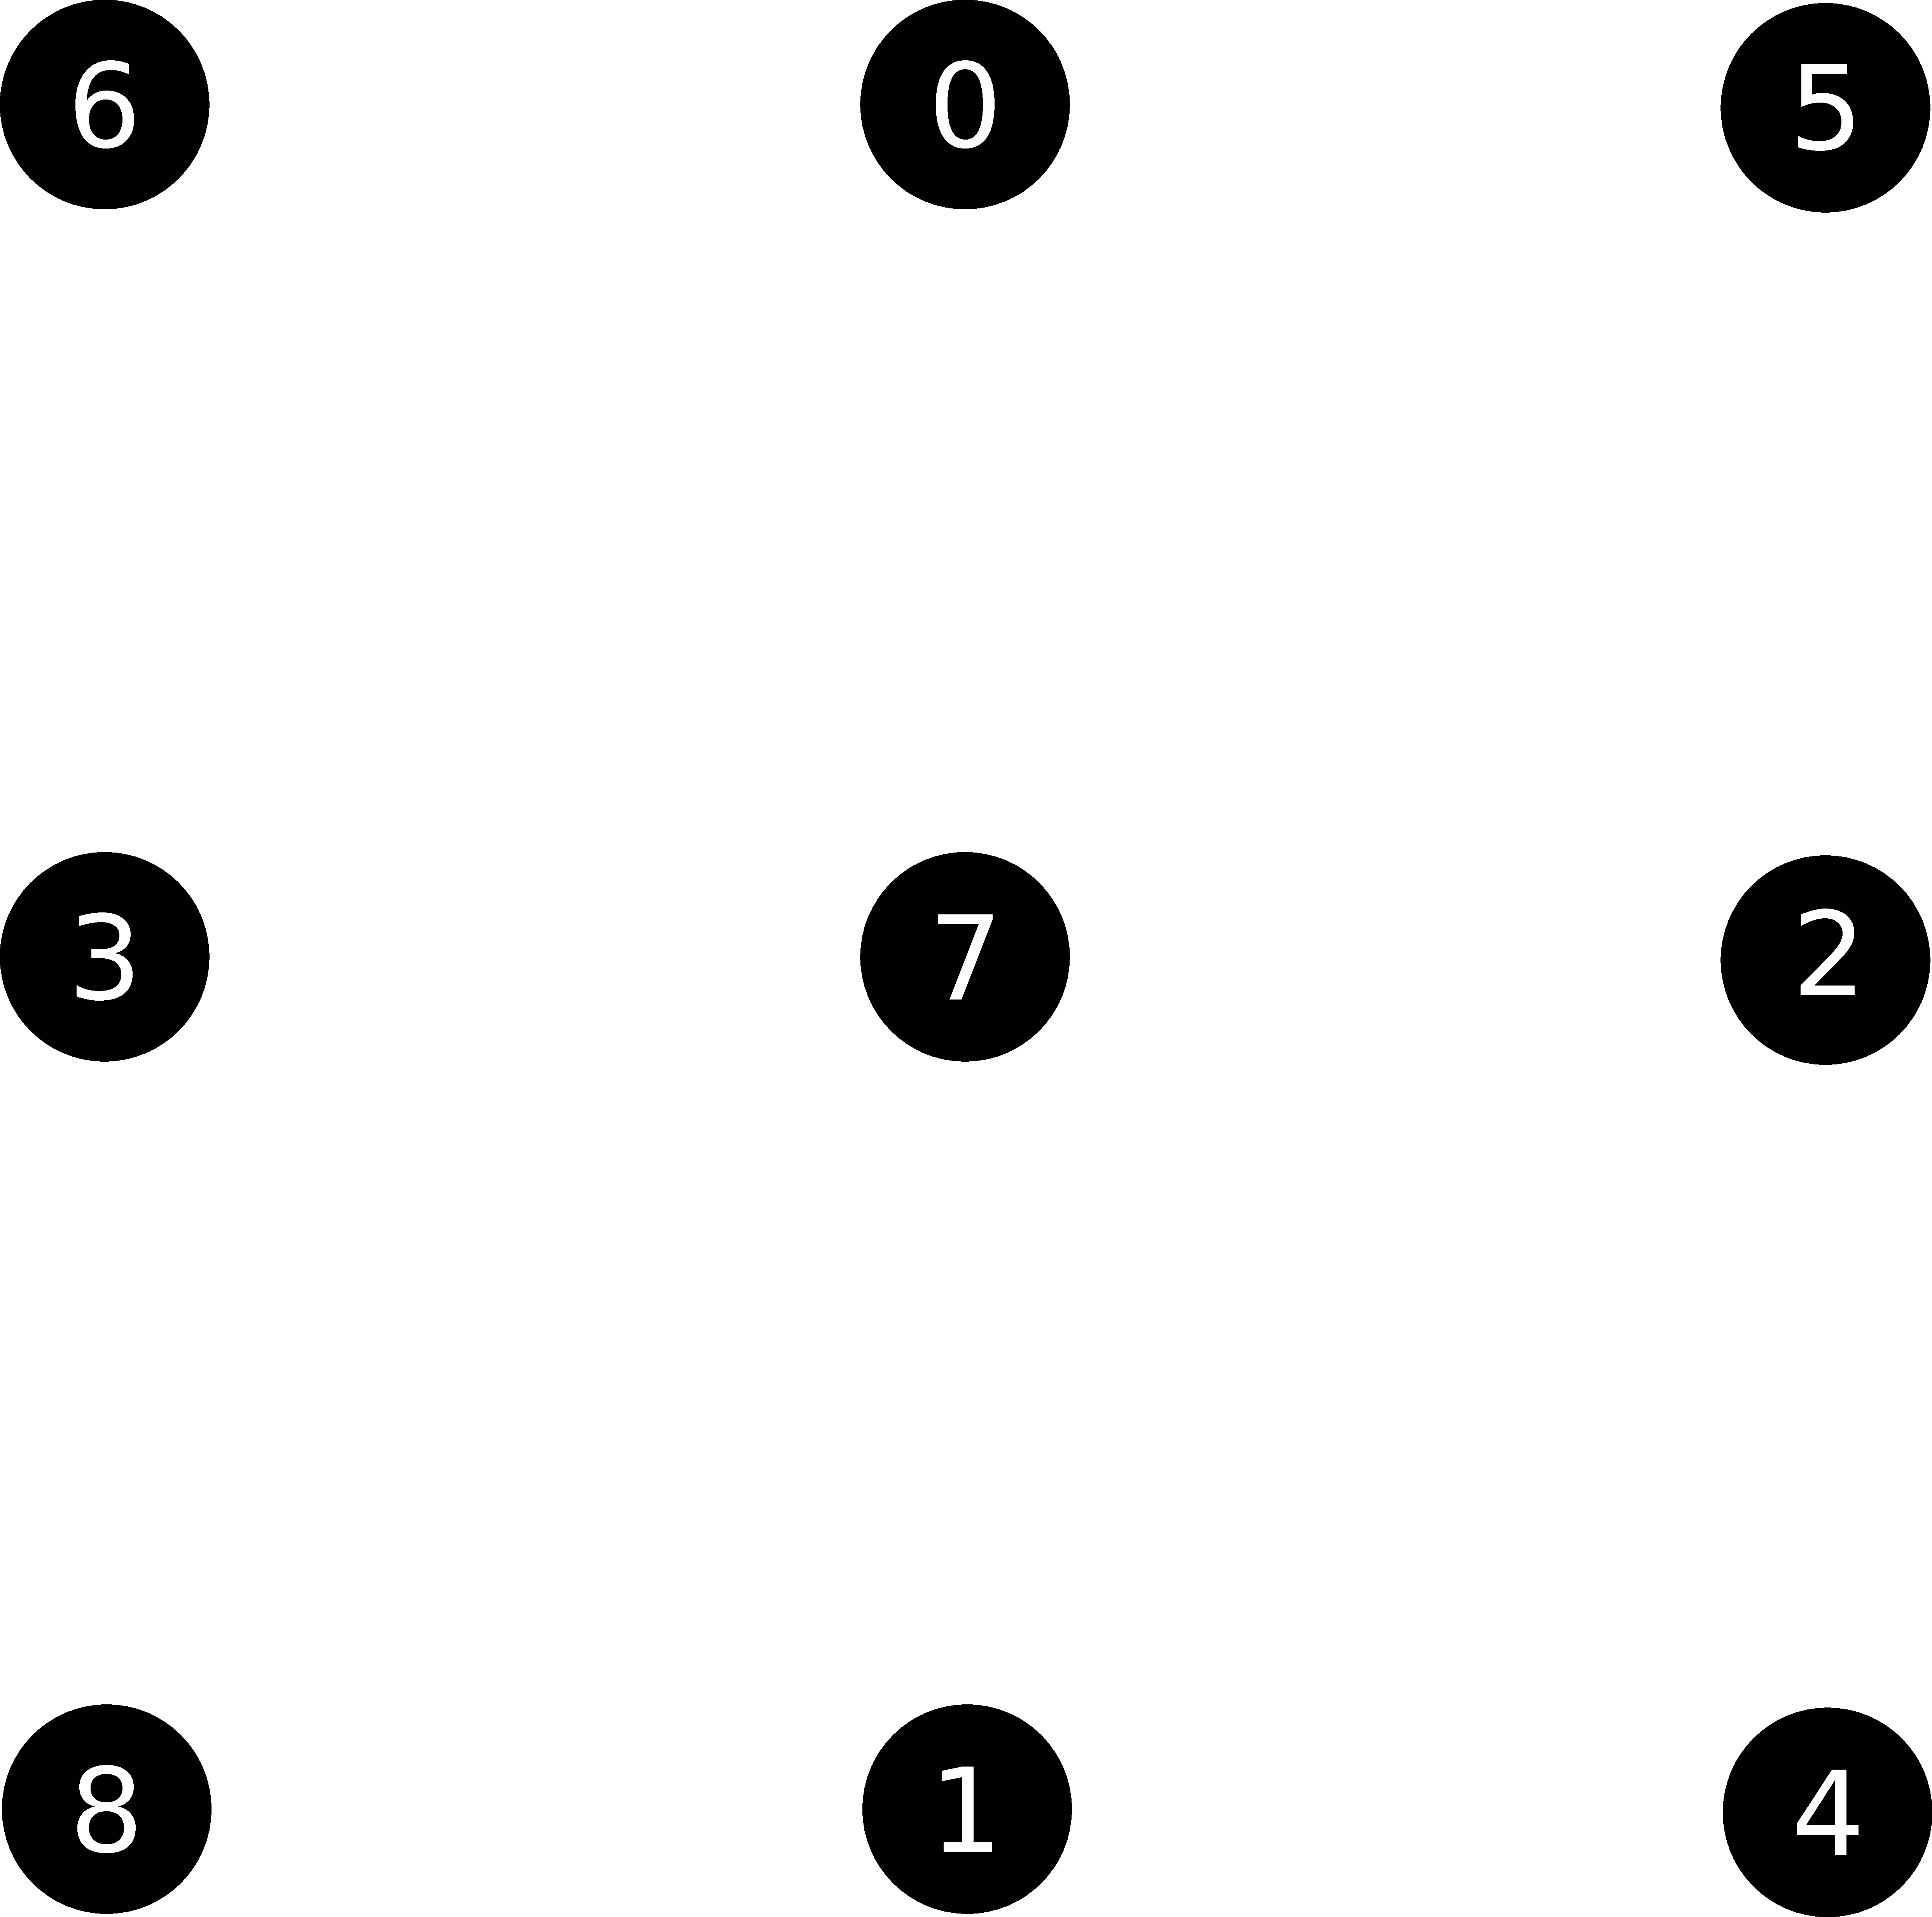
\includegraphics[scale=0.06]{./images/w3x3/w3x3-vertices.pdf}}}%
    \qquad \qquad \qquad
    \subfloat[Simplicial Mesh.]{{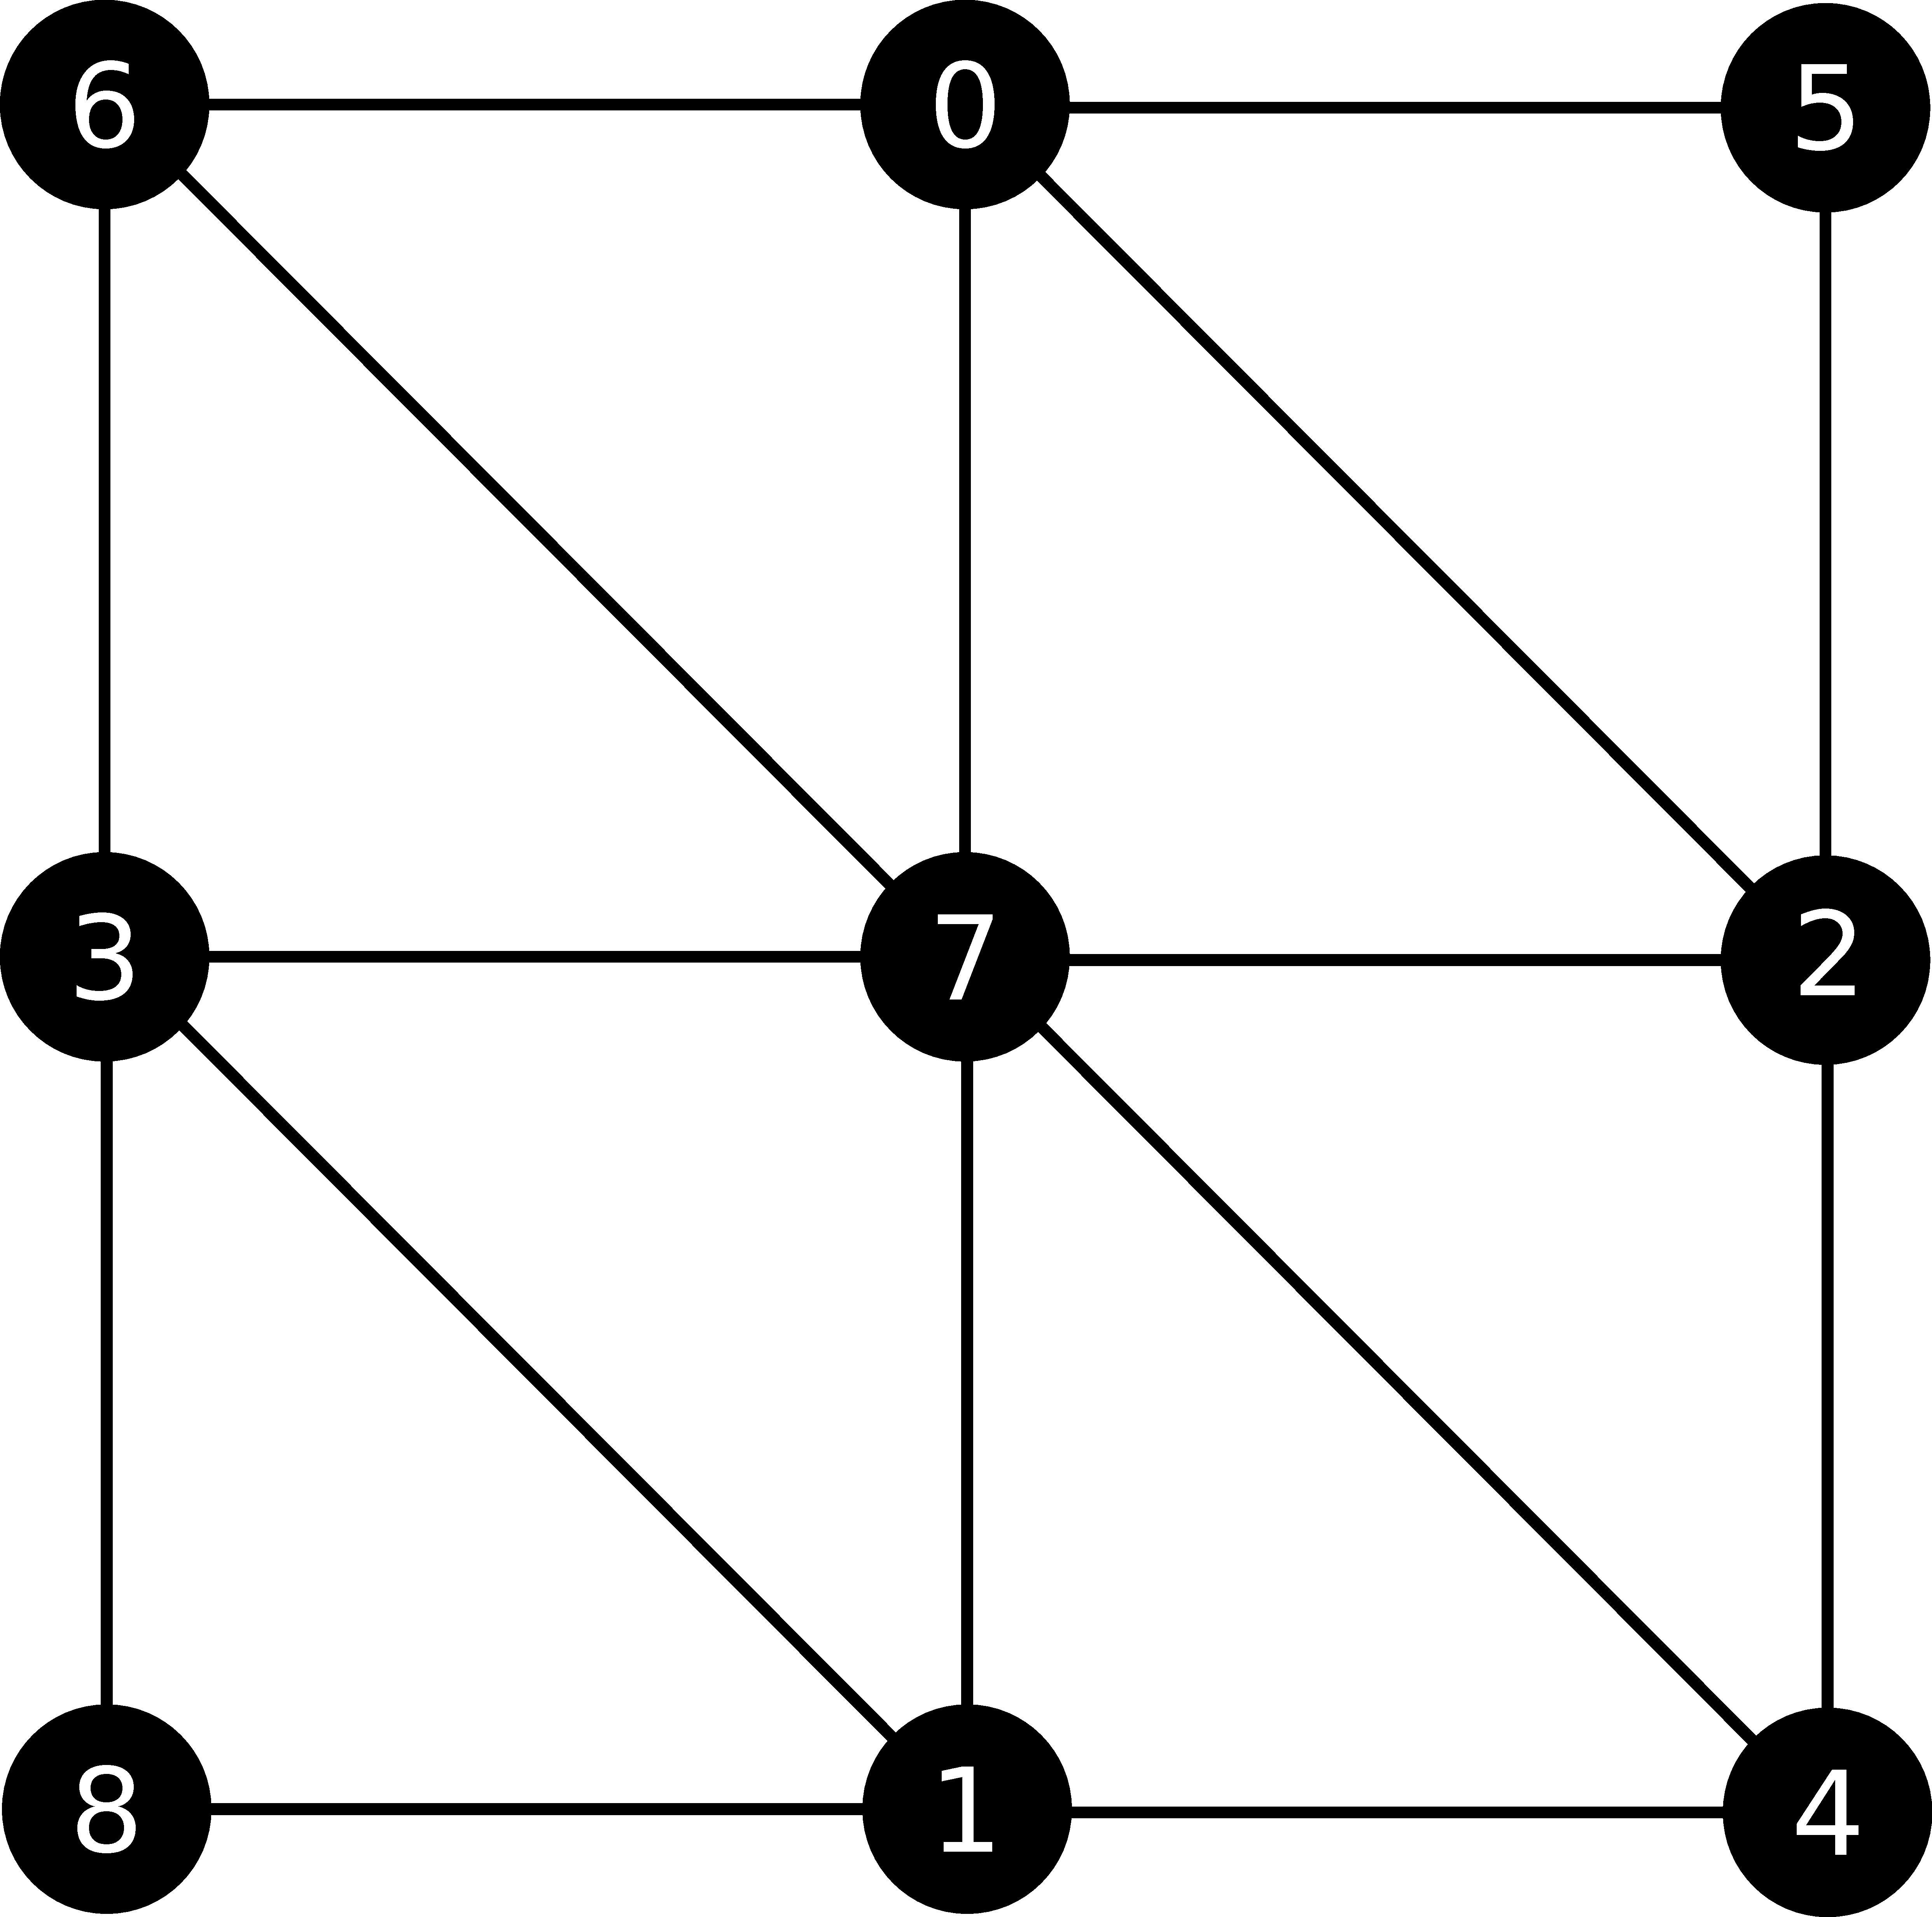
\includegraphics[scale=0.06]{./images/w3x3/w3x3-mesh.pdf}}}%
    \caption{Triangulation of input data to obtain a simplicial mesh.}%
    \label{fig:simplicial-mesh}%
\end{figure}
For simplicity and without loss of generality we will work with two-dimensional domains where the value samples are evenly spaced out in a grid-like fashion (Figure \ref{fig:simplicial-mesh}). The values of the approximation function at the simplicies are obtained via linear interpolation between the vertices of each simplex. As long as the original values we have sampled are unique it can be shown that the linear interpolation function is a Morse function and that all critical points are the vertices of the mesh \cite{curvature-embeded-polyhedra}.

\section{Existing Contour Tree Algorithms}


 % @TODO What about higher dimensions and expand parallel stuff?

The first efficient algorithm for constructing contour trees \cite{first-ct-algo} is due to Van Kreveld et al. Its running time is $O(NlogN)$ on two dimensional domains and $O(N^2)$ in higher dimensions where $N$ is the number of triangles in the simplicial mesh. Tarasov and Vyalyi \cite{second-ct-algo} extended this algorithm to work in time $O(NlogN)$ on three dimensional domains. Their approach however involved a complicated procedure for dealing with multi-saddle points. Both algorithms suffer from lack of generality and non-trivial treatment of multi-saddle points. Carr et. al \cite{ct-big-paper} introduced an algorithm with running time $O(nlogn + N\alpha(N))$ where $n$ is the number of vertices in the simplicial mesh and $\alpha$ is the notoriously slow growing inverse Ackerman function. This algorithm works in any number of dimensions and has simple treatment of multi-saddle points.

More recent developments in the field focus on extending the existing algorithms to accommodate the distributed \cite{distributed-ct-algo, distributed-ct-algo-2} and shared memory parallelism paradigms \cite{parallel-peak-pruning, parallel-ct-1}. The focus of this dissertation will be one of the latest developments in a data parallel shared memory algorithm for contour tree computation
\cite{parallel-peak-pruning}. Before introducing how that algorithm operates and one of the issues related to its parallel performance we will first give a more detailed overview of the most established serial algorithm \cite{ct-big-paper} on which the data parallel one is based on. In order to talk about any of the two algorithms we must establish some notation and define height graphs and trees as they are defined in \cite{carr-masters}.


\section{Height Trees}

A height graph is a graph $G = (V, E)$ together with a real valued function $h$ defined on the vertices of $G$. Height graphs are also known in the literature as weighted graphs. We are changing our notation to be more indicative of the fact that the weight function is defined on the vertices and that it corresponds to height of points in a simplicial mesh. A height tree is a height graph which is a tree. Contour trees are height trees because nodes in the contour tree correspond to nodes in the mesh and can inherit their height (sampled) value. Analogous to the assumption we have made about uniqueness of values we will also assume all vertices in the height trees we consider have unique heights. In other words $h(u) \ne h(v)$ for all $u ,v \in V(G)$ where $u \ne v$. The function $h$ naturally induces a total ordering on the vertices. From now on we will assume the vertices of $G$ are given in ascending order. That is to say, $V(G) = \{v_1, v_2, ... , v_n\}$ where $h(v_1) < h(v_2) < ... < h(v_n)$. This lets us work with the indices of the vertices without having to compare their heights directly. In this notation $h(v_i) < h(v_j)$ when $i < j$.

Introducing the height function allows us to talk about ascending and descending paths. A path in a graph is a sequence of vertices $(u_1, u_2, ... , u_k)$ where $u_i \in V(G)$ for $i \in \{1, 2, ..., k\}$ and $u_iu_{i+1} \in E(G)$ for $i \in \{1, 2, ..., k-1\}$. A path in a height graph is ascending whenever $h(u_1) < h(u_2) < ... < h(u_k)$. If we traverse the path in the opposite direction it would be descending. We will simply call these paths monotone whenever we wish to avoid committing to a specific direction of travel.

When working with height graphs it is useful to extend the definition of a degree of a vertex by taking the height function into account.

\begin{defn} Let $G$ be a height graph and $v$ a vertex of $G$. The up degree of $v$ is defined as the number of neighbours of $v$ with higher value. It is denoted as $\delta^+(v) = \big|\{ u \in N(v) : h(u) > h(v) \}\big|$.   \end{defn}

The down degree of a vertex $v$ is defined analogously as $\delta^-(v) = \big|\{ u \in N(v) : h(u) < h(v) \}\big|$. In the context of height trees the definitions of up and down degrees of a vertex allow us distinguish between two types of leaves - lower and upper leaves.
\begin{defn} Let $G$ be a height graph and $v$ a vertex of $G$. If  $\delta^+(v) = 1$ and $\delta^-(v) = 0$ then $v$ is a lower leaf.  \end{defn}

If $\delta^+(v) = 0$ and $\delta^-(v) = 1$ then $v$ is an upper leaf. We will see in the next section how differentiating between the two types of leaves is a critical part in the computation of the contour tree.

\section{Serial Algorithm}

The contour tree is a tree that consists of \cite{first-ct-algo}:

\begin{itemize}
    \item Vertices or supernodes that correspond to level sets that contain a critical point.
    \item Edges or superarcs correspond to path-connected regions bounded by two level sets which both contain a critical point. They connect the supernodes those level sets correspond to.
\end{itemize}

% @TODO Think about this contruction and destruction business
The contour tree contains information of two types of events - joining and splitting of contours. We can derive two other height trees from the contour tree that each contain the information of the joining and splitting events separately. These are called the join and split trees \cite{ct-big-paper}. The join tree contains information for the contours that join together and the split tree holds the information for the contours that split apart. The join tree of a contour tree summarises the evolution of the connectivity of the sublevel sets of the interpolation function and the split tree of the superlevel sets. You can find an example of the join and split trees of Figure \ref{fig:mesh-join-split-contour}.

% The two are symmetric in that the join tree of the function $f$ is isomorphic to the split tree of the negative of the function $-f$.

\begin{figure}[h]%
    \centering
    \subfloat[Simplicial mesh.]{{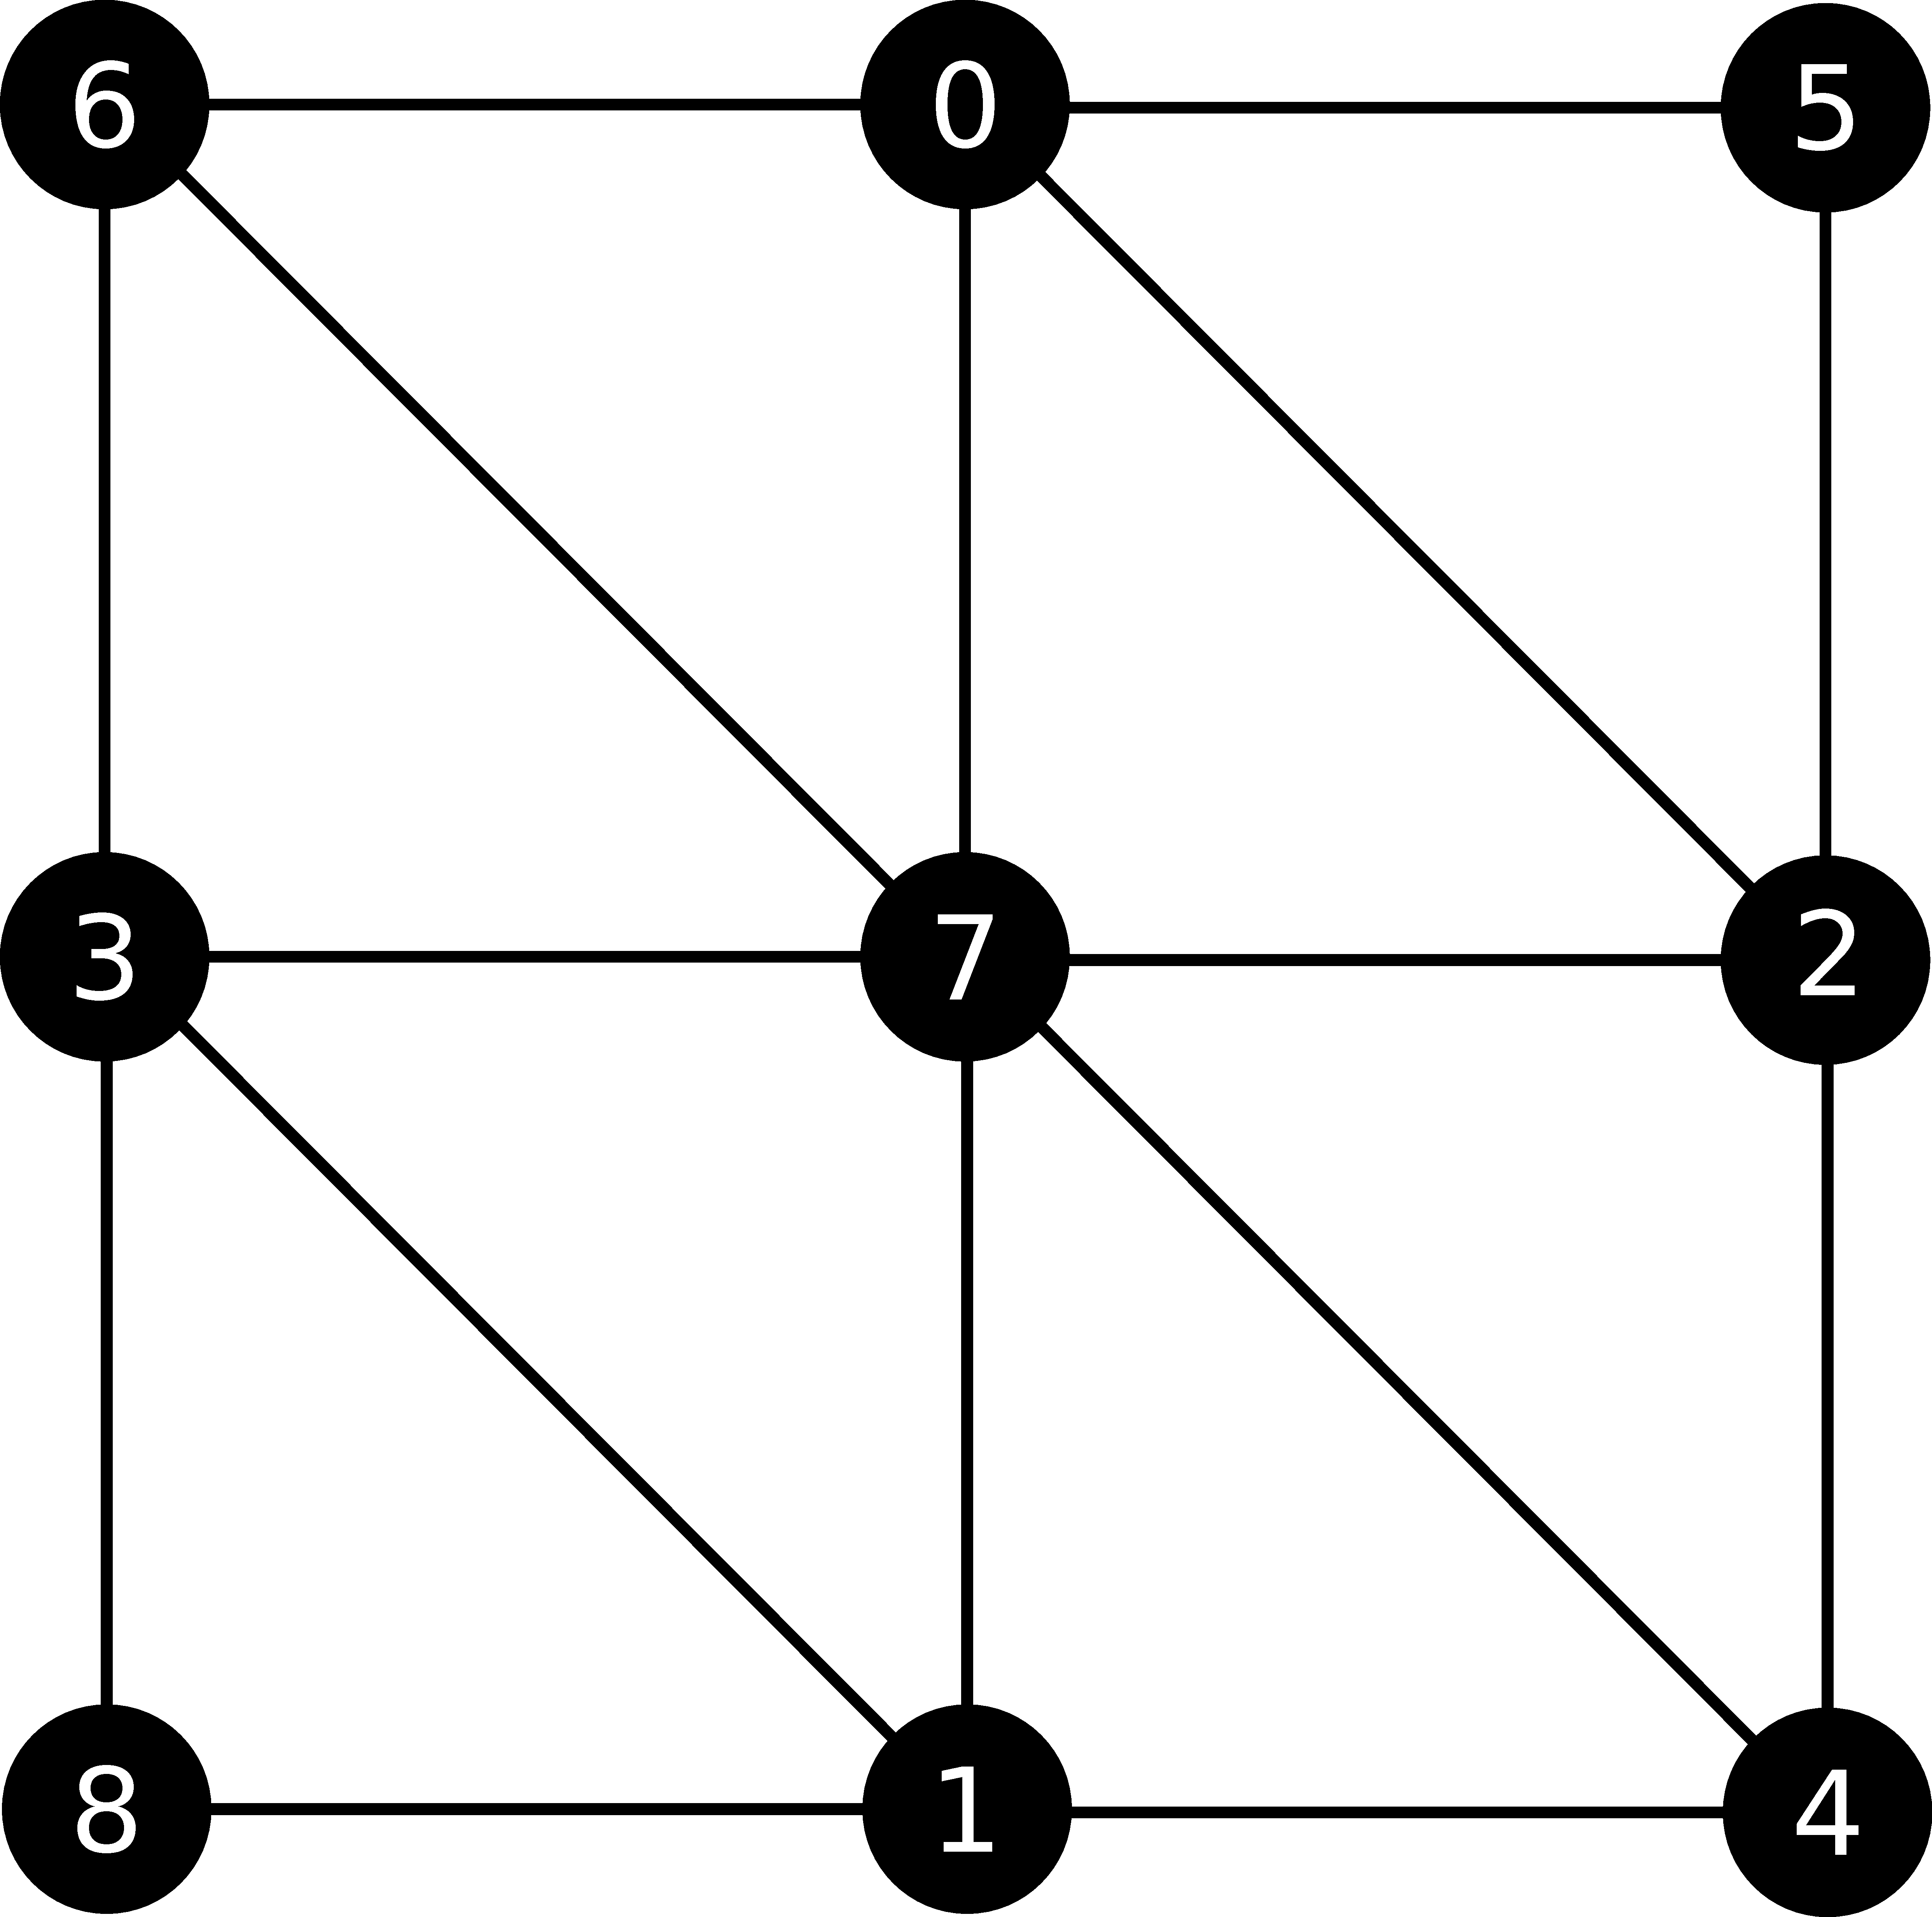
\includegraphics[scale=0.06]{./images/filtration/asc/x9.pdf}}}%
    \qquad \qquad \qquad
    \subfloat[Contour tree.]{{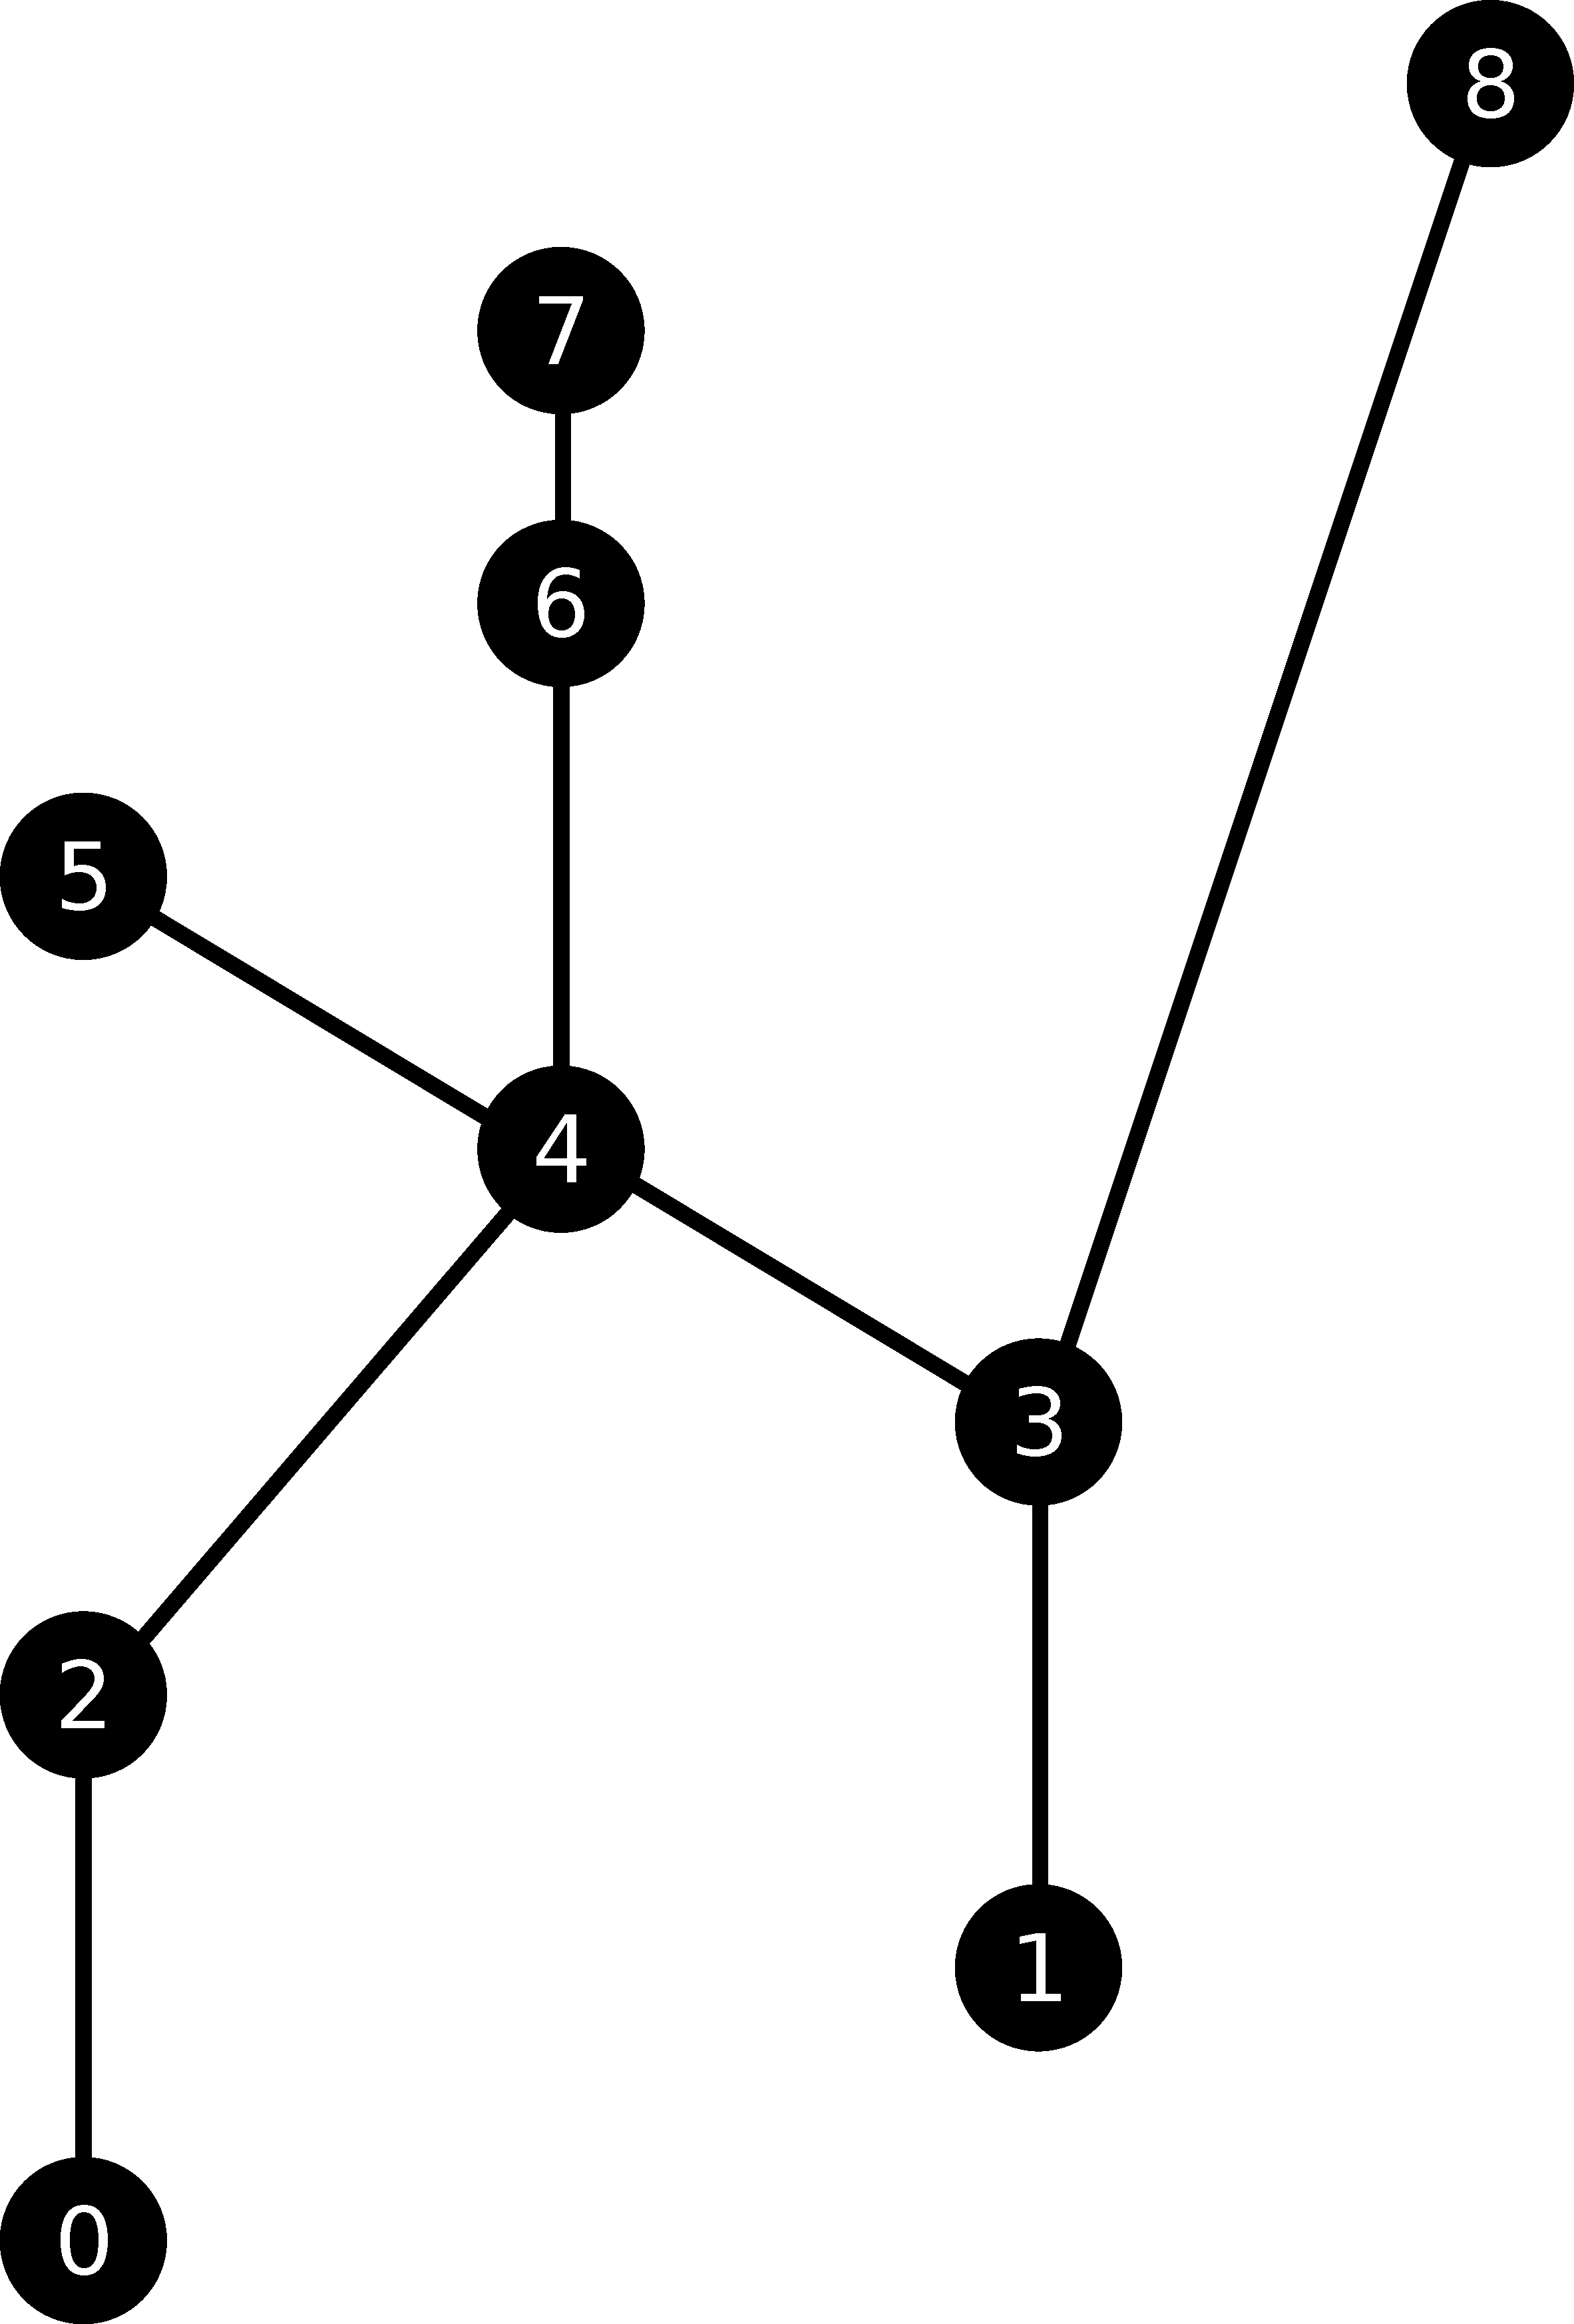
\includegraphics[scale=0.10]{./images/w3x3/w3x3-contour-tree.pdf}}}%
    \qquad \qquad \qquad

    \subfloat[Join tree.]{{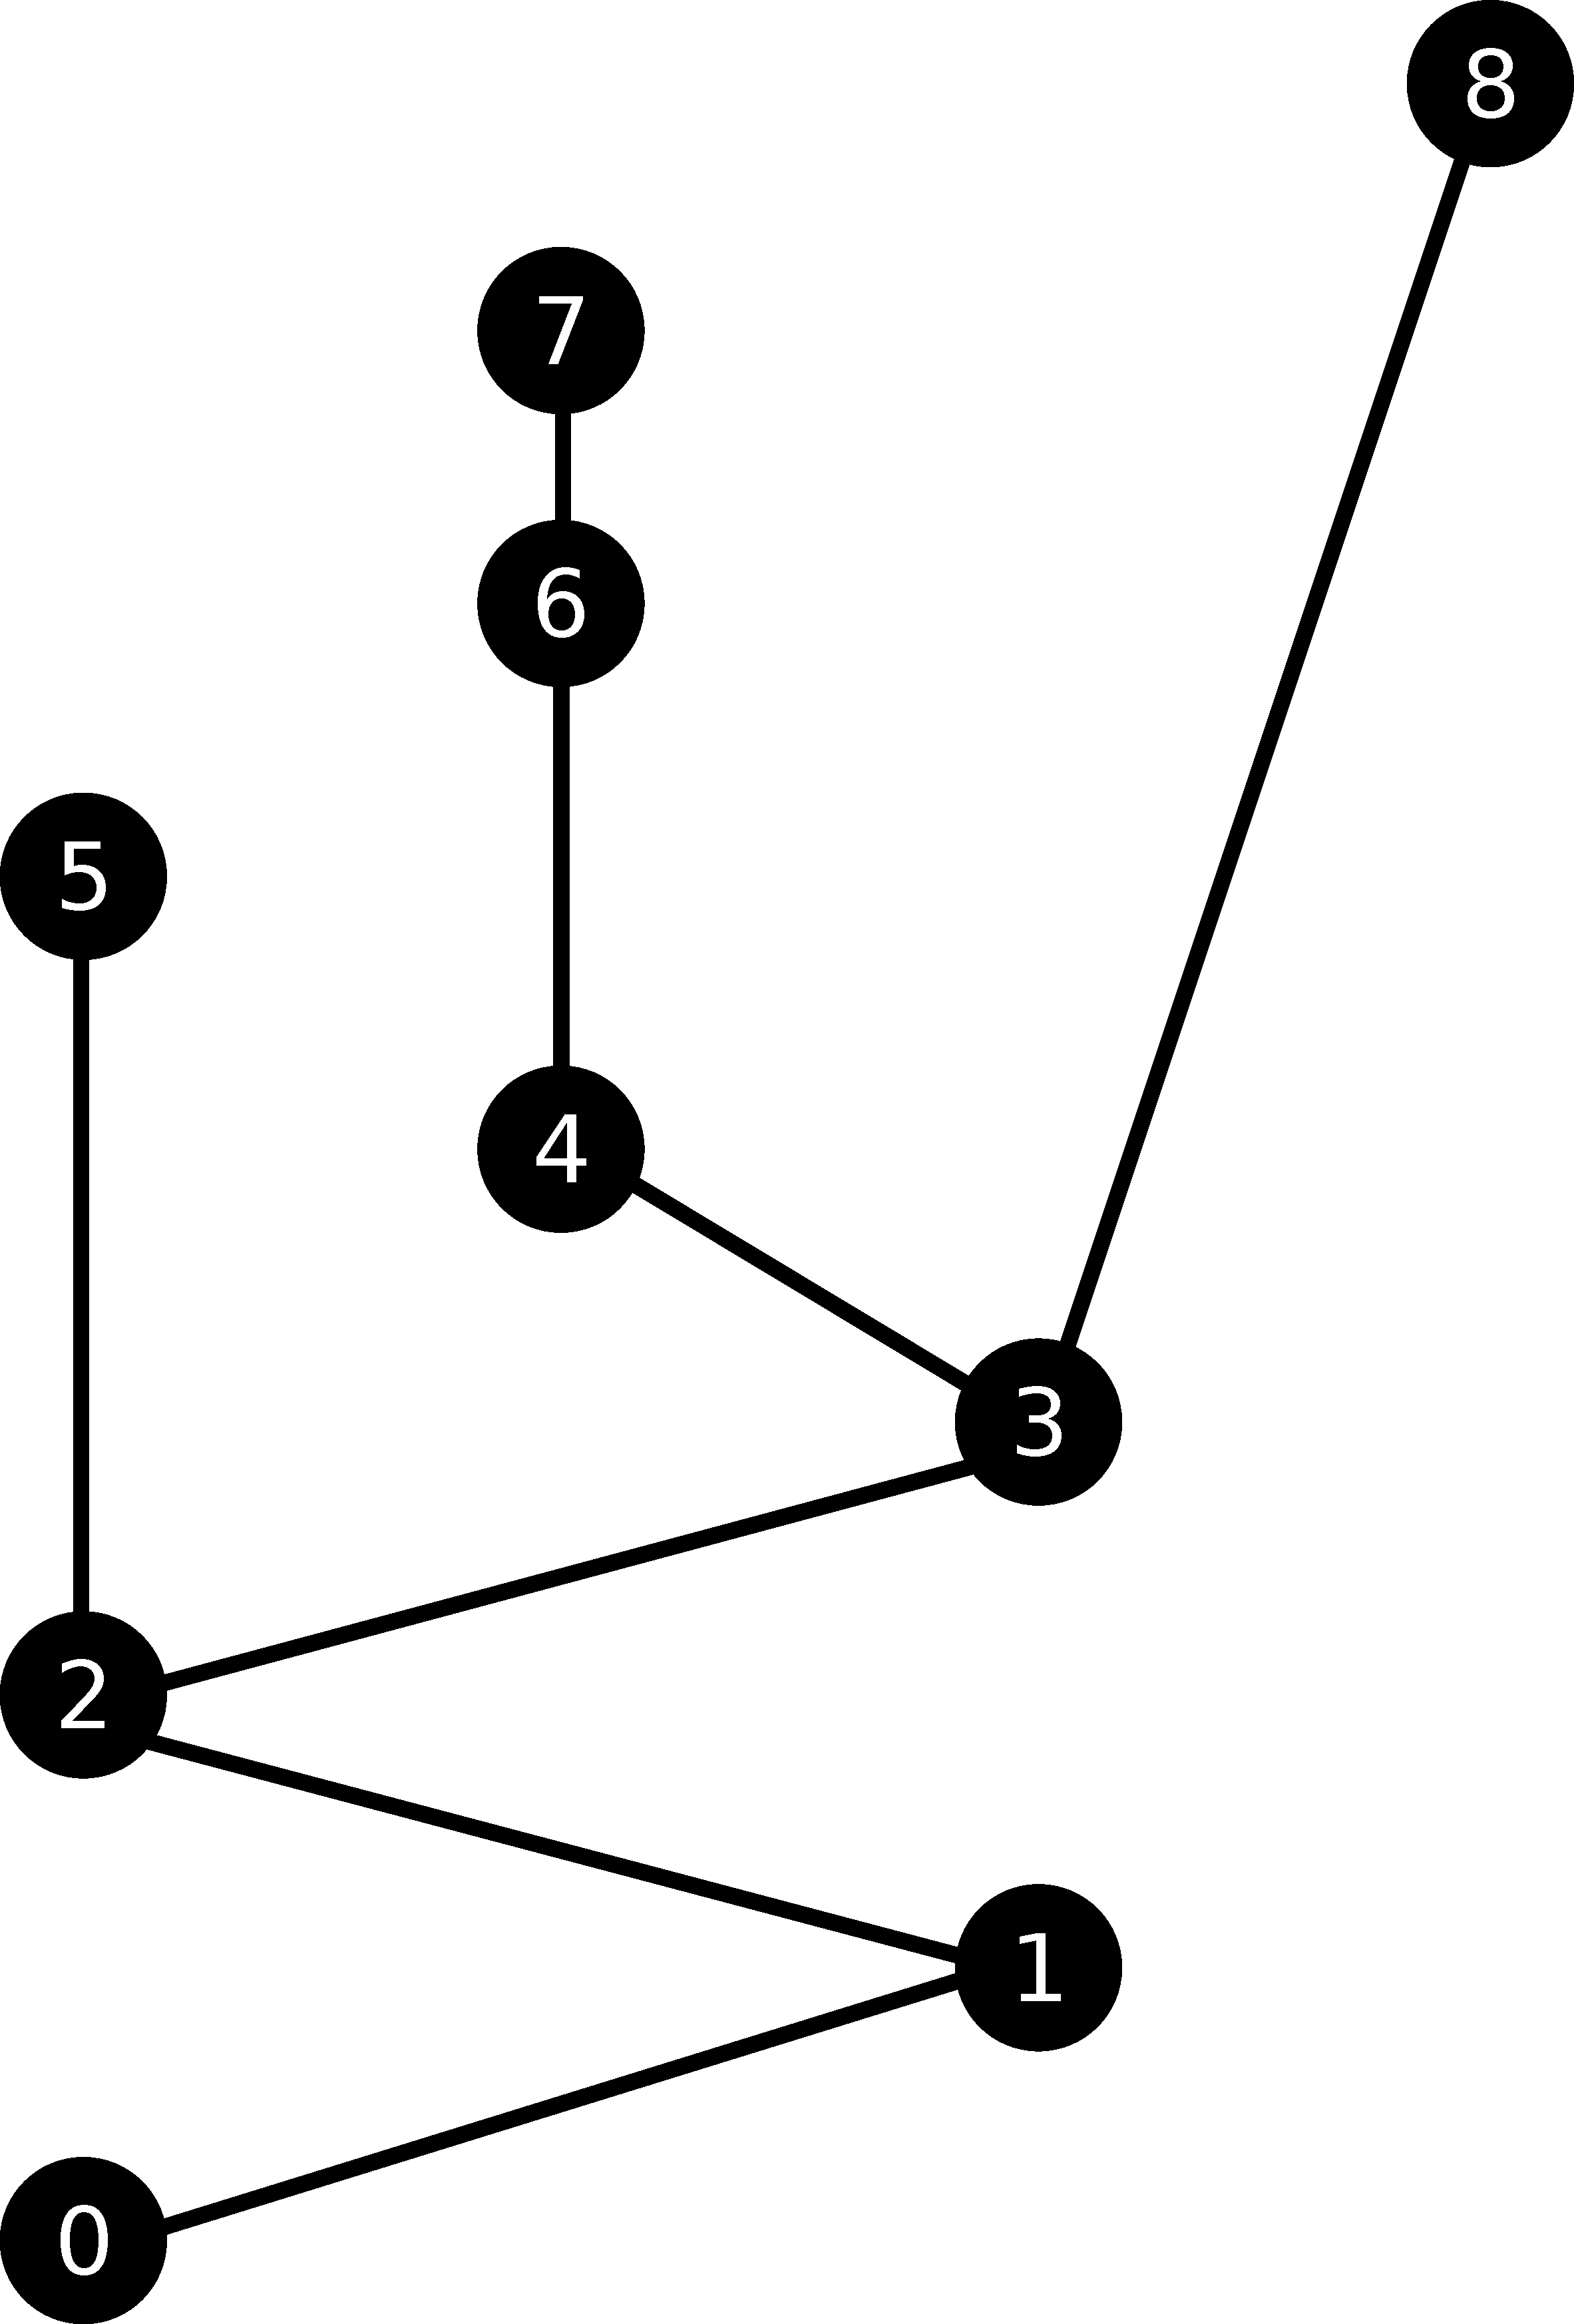
\includegraphics[scale=0.10]{./images/w3x3/w3x3-join-tree.pdf}}}%
    \qquad \qquad \qquad
    \subfloat[Split tree.]{{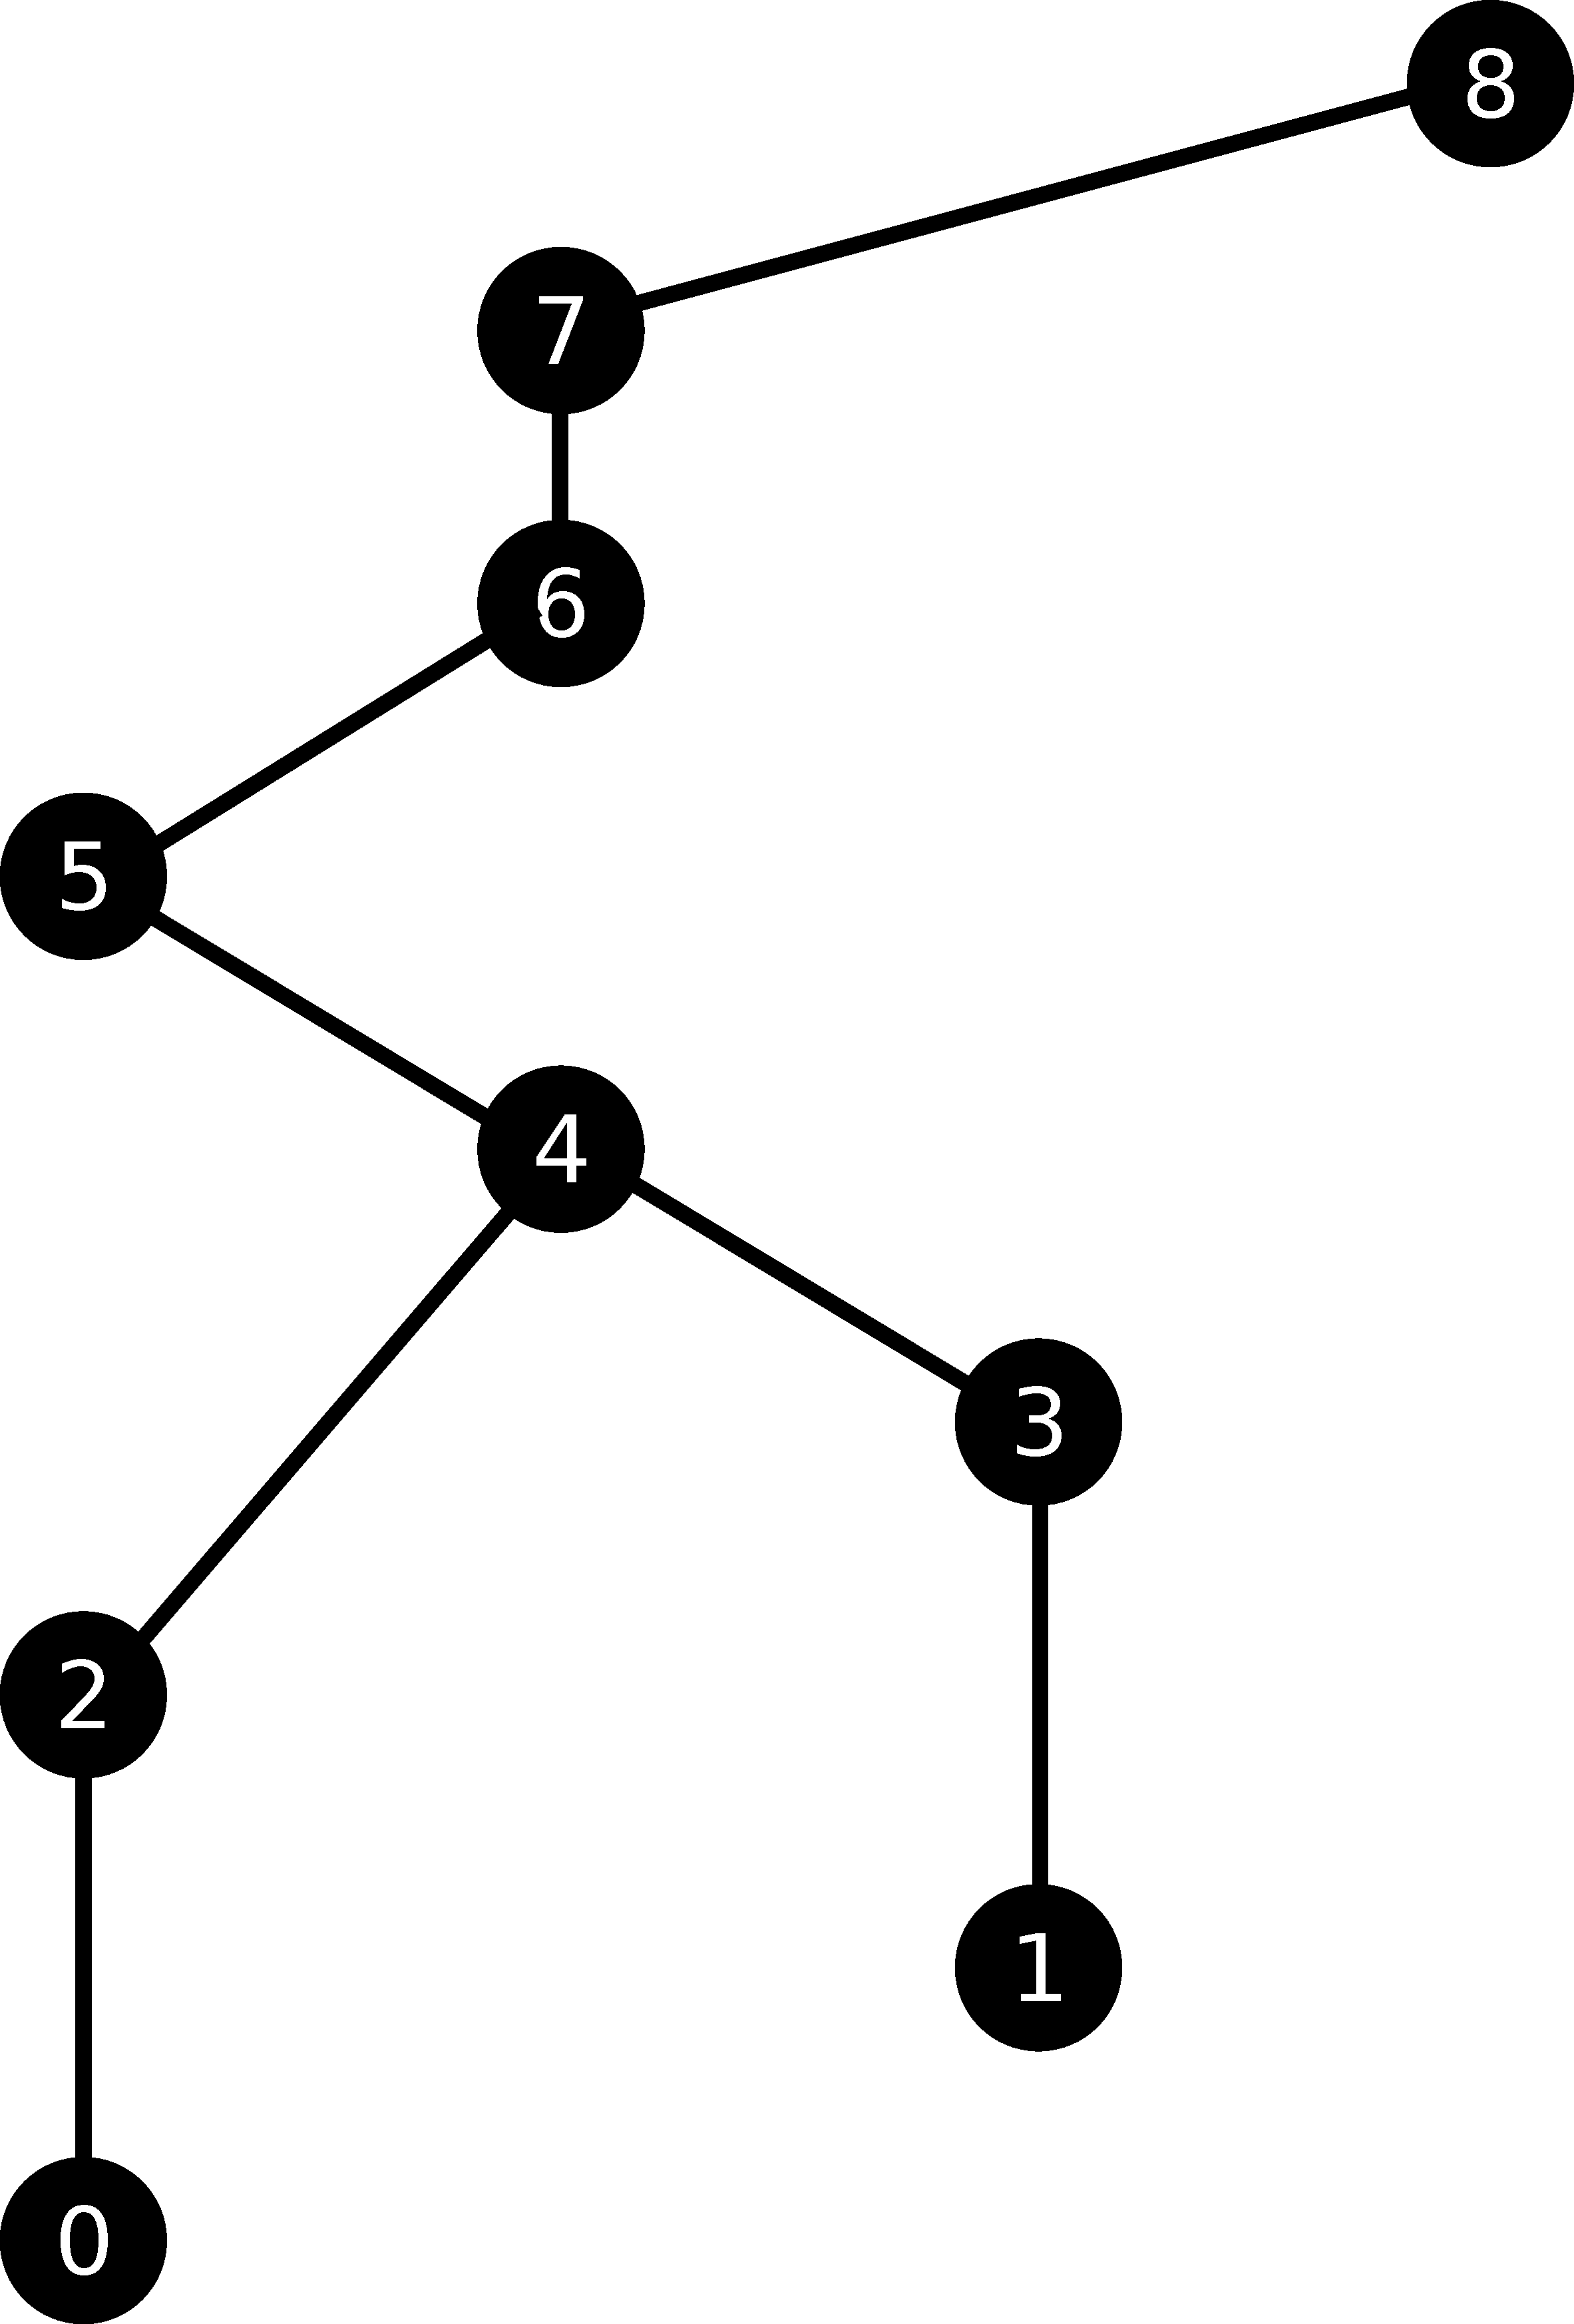
\includegraphics[scale=0.10]{./images/w3x3/w3x3-split-tree.pdf}}}%
    \caption{The simplicial mesh, join and split trees and contour tree.}%
    \label{fig:mesh-join-split-contour}%
\end{figure}

The reason we would like to study join and split trees is that the contour tree can be reconstructed from them. The core idea of the algorithm we will present is that we can derive the join and split trees directly from the simplicial mesh and then combine them to obtain the contour tree. We will first describe how the join and split trees are computed from the mesh. We only have to describe the process for the join tree because the computation of the split tree is symmetrical \cite{ct-big-paper}.

\begin{defn} A join component is a connected component in the superlevel set $f^{-1}([h, \infty))$ at some $h \in \mathbb{R}$.  \end{defn}

Let $M$ be the simplicial mesh from Figure \ref{fig:mesh-join-split-contour} (a) and let $h : M \to \mathbb{R}$ be the interpolation function defined on it. We will refer to $h$ as the height function. To construct the join tree we are going to have to keep track of which components merge together in the superlevel sets of $h$. We will consider all superlevel sets $M^t = h^{-1}([t, \infty)) = \{x \in M : h(x) \in [t, \infty) \}$ as a one parameter family $\{M^t\}_{t \in \mathbb{R}}$
of nested subsets of $M$. We can see from this definition that $M^a \subseteq M^b$ whenever $a \le b$. What the join tree captures is how the connectivity of the superlevel sets changes as the parameter $t$ is increased. The connectivity of superlevel sets changes either at local minima where a new component is created or a saddle point that merges two or more join components.

%We will not formalise the notion of tracking join components and constructing a join tree. Let us work in the general setting where $X$ is any path-connected topological space and $h : X \to \mathbb{R}$ is a function defined on $X$. The claims we make will hold in the special case where $X$ is a simplicial complex. Let us consider all sublevel sets $X_t = h^{-1}((-\infty, t]) = \{x \in X : h(x) \in (-\infty, t] \}$. They form a one parameter family $\{X_t\}_{t \in \mathbb{R}}$ of nested subsets where $X_a \subseteq X_b$ whenever $a \le b$. What the join tree captures is how the connectivity of the sublevel sets changes as the parameter $t$ is increased.

To visualise this process we can contract every join component to a point much like we did in the Reeb graph. The only difference here is that the equivalence relation is defined for all points in a superlevel set $h^{-1}([t, \infty))$ instead of a level set $h^{-1}(\{t\})$. Because of this change and because join components can only merge the join tree is a tree \cite{comp-topo}. Furthermore if $M_m = M$ is the last superlevel set for some $m \in \mathbb{R}$ then all join components merge into one because $M$ is path connected.

We will briefly outline the algorithm for constructing the join tree and refer the reader to \cite{ct-big-paper} for further implementational details. We know that all critical points are vertices of $M$ and that it is only at the critical points that changes in the topology of the superlevel sets can happen. The algorithm works by considering the vertices of the simplicial mesh in ascending order of their height. If the current vertex is a local minimum we directly add it in the join tree because it starts a join component. If the current vertex is a saddle that joins two or more components (join saddle) we add it to the join tree and add an edge between it and the local minima of the join components it merges. At the end of the computation all vertices will be in the same join component. In order to keep track of which join components different vertices belong to we can use the union-find data structure. The term  $\alpha(n)$ in the time complexity of the contour tree algorithm comes from the basic operations of find and search in the union-find data structure.

% @TODO Define Join Saddles and Subdivided edges
Not all vertices of the mesh will be in the join tree. Only those which correspond to local maxima and to join saddles. This will pose a problem later on when we wish to combine the join and split trees. To avoid this problem we can augment the join tree by adding all missing vertices. This is done through edge subdivision. Let $a \text{ and } b$ be two adjacent vertices in the join tree.  Let $\{v_1, v_2, ..., v_n\}$ be vertices in the mesh that are not in the join tree that are given in ascending order in terms of height.  Suppose that $h(a) < h(v_i) < h(b)$ for all $i \in \{1, 2, ..., n\}$ and the vertices $v_i$ are in the same connected component of $X_b - h^{-1}(\{b\}) = h^{-1}((-\infty, b))$. In order to augment the join tree with the first vertex we subdivide the edge $ab$ and label the new vertex as $v_1$. Next we subdivide $v_1b$ and label the new vertex as $v_2$. We continue to do so and on the $k$th step we subdivide the edge
$ v_{k-1}b $ and label the new vertex as $v_k$  .

The procedure of augmentation can be applied to the split tree and contour tree as well. We can use it to augment the contour tree with all vertices of the mesh which are not critical points. This is why we will differentiate between the contour tree and the augmented contour tree. The augmented contour tree contains all regular vertices of the simplicial mesh.

The second step of the algorithm is to combine the join and split trees to produce the contour tree. We will actually combine the augmented join tree with the augmented split tree to obtain the augmented contour tree. Removing the augmentation of the contour tree is left as an optional final step. The first step in merging the two is to identify all leaves of the contour tree and their incident edges. We can recognize them immediately from the join and split trees using the following property \cite{carr-masters}.

\begin{property} Let $v$ be a vertex such that its up degree in the join tree is $0$, its down degree in the split tree is $1$ and $u$ is its only down neighbour in the split tree. Then $v$ is an up leaf in the contour tree and $vu$ is an edge in the contour tree.  \end{property}

There is an analogous property in the case of down leaves and their adjacent edges.

\begin{property} Let $v$ be a vertex such that its up degree in the join tree is $1$, its down degree in the split tree is $0$ and $u$ is its only down neighbour in the join tree. Then $v$ is a down leaf in the contour tree and $vu$ is an edge in the contour tree.  \end{property}

Now suppose that we have identified $v$ as a leaf and $vu$ as its adjacent edge in the split or join tree. Another property \cite{carr-masters} tells us that if we perform vertex contraction on $v$ (remove $v$ and form a clique from its neighbourhood) from the join, split and contour trees we obtain the join and split trees of the contour tree with $v$ removed. This allows us to iteratively remove leaves from the join and split trees, add them to the contour tree and then delete them from the join and split tree. We can repeat this process until we have removed all vertices from the join and split trees and all vertices are present in the contour tree. For a detailed description of this process we refer the reader to \cite{ct-big-paper}.

 % We are allowed to do so because removing all leaves in a tree leaves the tree with at least one leaf if it is not empty where the algorithm will terminate.

The Serial algorithm for the construction of the contour tree is a summary of the results we have obtained so far:

\textbf{Step 1.} Read input data and convert it to a simplicial mesh.

\textbf{Step 2.} Compute the augmented join and split trees from the simplicial mesh.

\textbf{Step 3.} Iteratively remove leaves from the augmented join and split trees and add them to the augmented contour tree until the augmented join and split trees are empty.

\textbf{Step 4.} Remove regular vertices from the augmented contour tree by contracting them.

\section{Parallel Algorithm}

The data parallel contour tree algorithm \cite{parallel-peak-pruning} is largely based on the serial contour tree algorithm we just described. The parallel approach borrows the two phase methodology of computing the join and split trees and then merging them. We will omit describing the process of parallelising join/split tree computation because it is not directly related to the issue we aim to address. We will describe how the merge phase is parallelised in detail.

The data-parallel paradigm works best when there are a large number of computational tasks to be carried out independently. Dependant tasks require some form of synchronisation. Synchronisation is costly in terms of performance. Removing a leaf in the merge phase of the serial algorithm requires little synchronisation with other vertices because it is a local operation. It only involves a few of the vertices of the join and split trees. This means that once we identify all up and down leaves we can remove them in parallel in a single iteration. The key problem to solve in the merge phase is to reduce the number of total iterations needed to remove all vertices from the join and split trees. The amount of parallelism in this computation is limited by the number of leaves at each iteration. For example a tree which is a path of length $n$ will take at least $n/2$ iterations and a tree with one central vertex and $n$ leaves adjacent to it will take only two iterations.

In a graph with no vertices of degree two at least half of the vertices are leaves (see Appendix \ref{chapter-proofs}). If at every iteration half of the remaining vertices are leaves the total number of iterations would be logarithmic in the number of vertices in the contour tree. In order to ensure this logarithmic collapse Carr et. al \cite{parallel-peak-pruning} have come up with a way of batching some of the paths that start at a leaf and consist of vertices of degree two, in a single iteration. We will call such paths leaf chains. The process of removing them in a single iteration is in effect equivalent to contracting all vertices in the tree of degree two. This leaves only leaves and vertices of degree three or higher and ensures the logarithmic collapse.

The main issue that arises is that leaf chains which are not monotone paths canno be processed in a single iteration. They require multiple iterations to process. When some of the vertices in the leaf chains have alternating height and we plot them according to their height they form a characteristic zigzag pattern. We will call paths W-Structures. See for example the path $(5, 2, 4, 3, 8)$ in the contour tree on Figure \ref{fig:mesh-join-split-contour}. These w-structures are the core issue we are addressing in this dissertation. We would like to obtain a better understanding of them and how and why they affect computation. The first step to solving such a problem is understanding it. The next chapter will address this by developing algorithms that analyse contour trees and determine the largest w-structures that is present in them.

% The issue arises from batching monotone paths is not a monotone path and some of the vertices inside it have alternating height. The we can only batch monotone subpaths and not the whole path. The more zig zags there are in the path the less monotone paths there and the more iterations we will require. This effectively serialises computation along them.

The theoretical issue caused by the w-structures becomes evident in the algorithmic analysis of the parallel contour tree algorithm. According to that the key question in the merge phase of the algorithm is how many iterations are needed to collapse the contour tree. Each iteration takes $O(1)$ steps, because all leaves can be processed in parallel, and $O(t)$ work, where $t$ is the number of leaves. This leads to an overall complexity of $O(log(t))$ steps and $O(tlog^2(t)$ work if we assume that no w-structures are present. If however there is a w-structure with more zigzags than $log(t)$ then the authors of the paper claim that the best formal guarantee they can give for the steps is the diameter of the contour tree. One of our goals in analysing the w-structures is to provide a better bound than the diameter of the tree. We will demonstrate how this can be done by developing some new theory about the w-structures in Chapter 4 and through an empirical analysis in Chapter 7.


\section{Contour Tree Simplification}

Finally we will introduce the topic of contour tree simplification. A central problem in using contour trees in visualisation is simplifying their output and presenting only the most important parts to enable human comprehension. The complexity of a contour tree of a large enough data set could severely limit its use. This is why it is vital to employ techniques that simplify the contour trees by removing parts of them that correspond to less "significant" topological features or sampling noise and error. This process helps to reveal the fundamental topological structures present in data.

% The most recent extensions of this work introduce high quality topological simplification [4] where the contour tree is pruned incrementally to reduce its complexity and highlight the fundamental structures present in the data.

% @TODO Add hamish phd thesis as generalisation?

One technique for contour tree simplification is branch decomposition \cite{ct-branch-decomp}. Branch decomposition involves decomposing the contour tree into a set of edge-wise disjoint monotone paths (branches) which cover all edges of the tree. The trivial branch decomposition of any tree is obtained by taking every edge to be a separate branch. A branch decomposition is hierarchical when there is exactly one branch that connects two leaves and every other branch connects a leaf to an interior node. An example of a hierarchical branch decomposition is shown in Figure \ref{fig:branch-decomp}.

The branches in this scheme represent pairs of critical points. This pairing of critical points forms the basis for a topological simplification. The topological simplification consists of removing branches that do not disconnect the tree. This produces a hierarchy of cancellations like in Figure \ref{fig:branch-decomp}. We define the persistence of a branch to be the bigger of the difference between its end points and the persistence of its children. Branches of high persistence reflect more prominent features in the tree. We apply the simplification by removing branches with low persistence that do not disconnect the tree.

The algorithm for producing the hierarchical branch decomposition of a contour tree is the following:

\begin{itemize}
    \item Identify all upper leaves that connect via branches to upwards saddles (merging of components).
    \item Identify all lower leaves that connect via branches to downwards saddles (splitting of components).
    \item Those pairs of leaves and saddles are the candidate branches. We pick the one with the lowest persistence (difference of height between the leaf and the saddle).
    \item Remove all vertices in the branch without the saddle.
    \item Continue this process until a single branch that connects two leaves is all that remains. That is the root branch.
\end{itemize}

For example let us construct the hierarchical branch decomposition of the contour tree from Figure \ref{fig:mesh-join-split-contour}. The first two candidate branches we identify are $(5, 2)$ with persistence $3$ and $(3, 8)$ with persistence $5$. We take the branch with lower persistence $(5, 2)$. In the next step the candidate branches are $(0, 4)$ with persistence $4$ and $(3, 8)$ with persistence $5$. We will take $(0, 4)$.
Afterwards the remaining candidate branches are $(3, 7)$ with persistence $4$ and $(3, 8)$ with persistence $5$. After removing $(3, 7)$ in the final stage the only remaining branch is $(1, 8)$. It is the root branch because it connects two leaves.
The produced pairs of critical points are $(2, 5), (0, 4), (3, 7)$ and $(1,8)$.

\begin{figure}%
    \centering
    \subfloat[Branch decomposition.]{{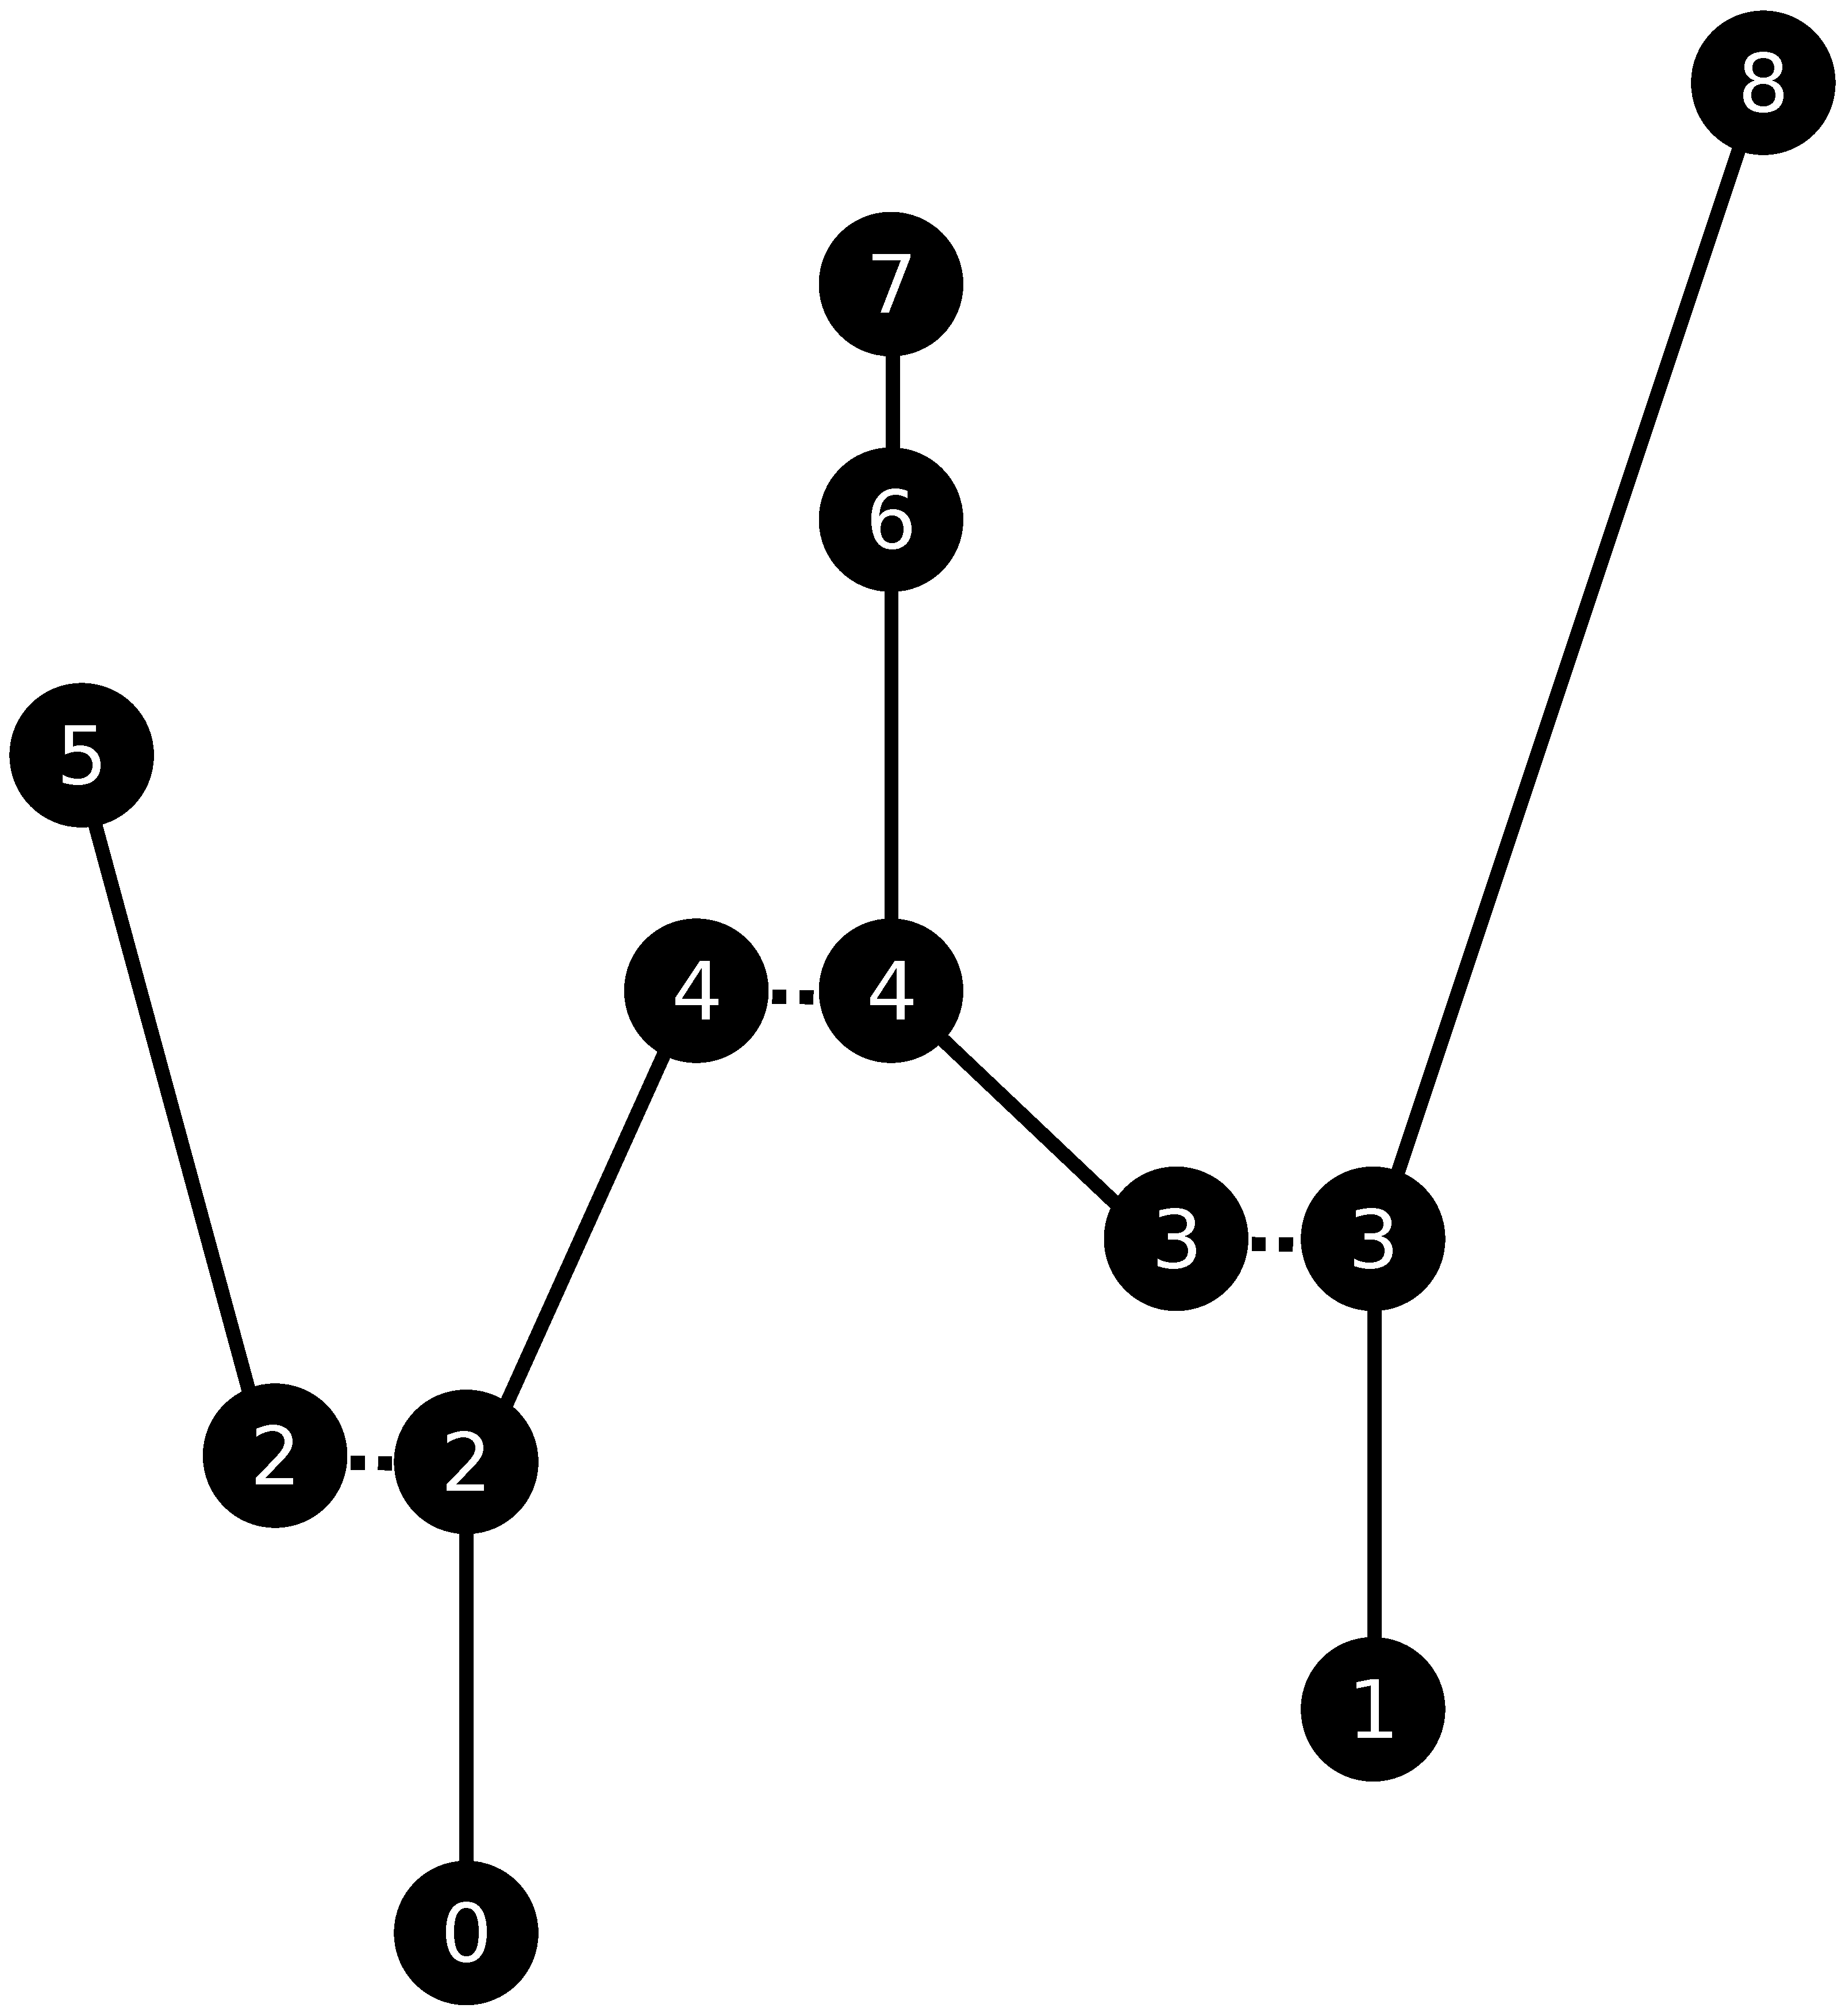
\includegraphics[scale=0.10]{./images/w3x3-ct-decomp.eps}}}%
    \subfloat[Heirarchical view of the branches.]{{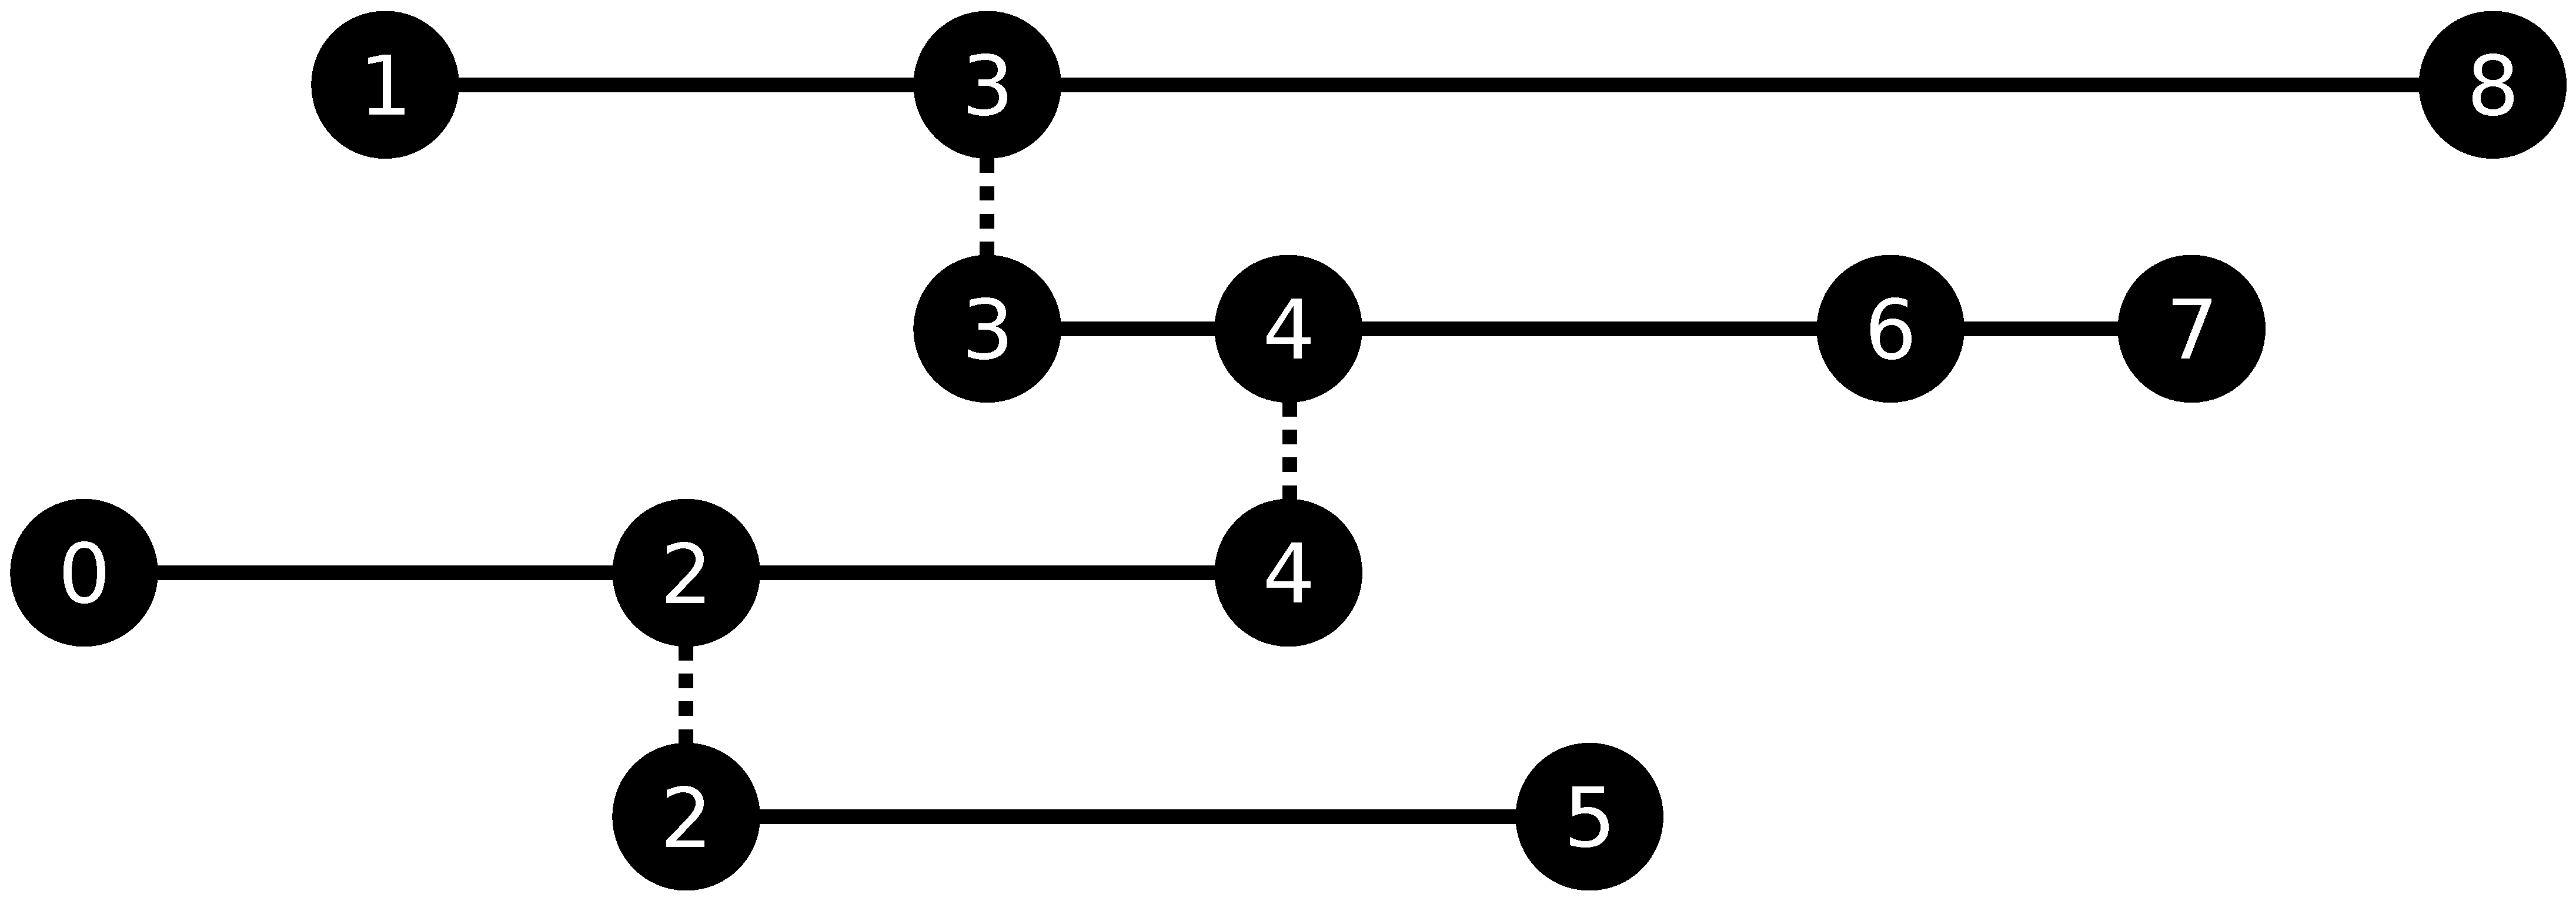
\includegraphics[scale=0.11]{./images/w3x3-ct-h-decomp.eps}}}%
    \caption{Hierarchical branch decomposition of the contour tree from Figure \ref{fig:mesh-join-split-contour} b.}%
    \label{fig:branch-decomp}%
\end{figure}

In the future we will omit the use of hierarchical and just refer to it as branch decomposition. Branch Decomposition is a form of topological simplification whose use is limited to the contour trees. In Chapter 6 we will present a more general topological simplification framework called persistent homology. Our goal will be to express branch decomposition in the framework of persistent homology and determine whether the two are equivalent.

% @TODO Todo talk about how this is used to remove noise and artifacts in data.

% @TODO Remove Stay Tuned
% The paper \cite{ct-branch-decomp} cites that the persistence defined in that way is similar to persistence first defined in \cite{persistence-original}. In Chapter N of this dissertation we will demonstrate that this claim is either incorrect of misleading. Stay tuned folks.


%Adds References to the table of content
%all you bibtex enteries go in the file called refs.bib
\addcontentsline{toc}{chapter}{References}
\bibliography{refs}

%any appendices you have go in a file called appendix.
\begin{appendices}

% \chapter{Additional Proofs}
%
% \begin{lem} In a tree with no vertices of degree two at least half of the vertices are leaves. \end{lem}
%
% \begin{proof}
%     Let $T = (V, E)$ be a tree with no vertices of degree two and let $L \subseteq V$ be the set of all leaves. As all leaves have degree one we have that $L = \{u \in V: d(u) = 1\}$. Furthermore for any tree we know that $|E| = |V| - 1$. Let us now use the handshake lemma:
%
%     $$ \sum_{u \in V}{d(u)} = 2|E| = 2(|V| - 1) = 2|V| - 2.$$
%
%     We will not separe the sum on the leftmost hand side of the equation in two parts. One for the vertices vertices in $L$ and one for the vertices in $V\textbackslash L$.
%
%
%     $$ \sum_{u \in L}{d(u)} + \sum_{u \in V\textbackslash L}{d(u)} = 2|V| - 2.$$
%
%     All the vertices in $L$ are leaves. By definition the degree of a leaf is one. Therefore $\sum_{u \in L}{d(u)} = |L|$. This leads us to the following:
%
%     $$  |L| + \sum_{u \in V\textbackslash L}{d(u)} = 2|V| - 2$$
%     $$  |L|  = 2|V| - 2 - \sum_{u \in V\textbackslash L}{d(u)}.$$
%
%     There are no vertices in $T$ of degree two and all vertices of degree one are in $L$. This means that all vertices in $V \textbackslash T$ have degree at least three. We can conclude that:
%     $$\sum_{u \in V\textbackslash L}{d(u)} \ge \delta(T - L).|V\textbackslash L| = 3(|V| - |L|) $$
%
%     Combining this with the previous equation we obtain that:
%
%     $$  |L| \le 2|V| - 2 - 3(|V| - |L|)$$
%     $$  |L| \le 2|V| - 2 - 3|V| + 3|L|$$
%     $$  -2|L| \le -|V| - 2$$
%     $$  |L| \ge \frac{|V|}{2} + 1$$
%
%     Which is exactly what we set out to proove.
%
%
% \end{proof}
%
% \begin{lem} There are at least $k$ vertices for every vertex of degree $k$ in a tree. \end{lem}
%
% \begin{proof}
%     Let $T$ be a tree and $u \in V(T)$ be a vertex in it. As any tree can be rooted, let us root $T$ at $u$ and call the new directed tree $T_u$. Let $U = \{u_1, u_2, ..., u_k\}$ be the neighbours of $u$. For each $u_i \in U$ if $u_i$ is not a leaf let $u_i$ be one of it's children. Repeat this process until every $u_i$ is a leaf. This is possible because $T$ is finite. All of the $u_i$ are distinct, for otherwise there would be a cycle in $T$.
%
% \end{proof}
%
%
% \chapter{Vector Spaces, Quiver Diagrams and Barcode Diagrams}
%
% *This chapter will probably be redistributed in the homology chapter. I'll probably remove it.*
%
% Should I define a vector space, bases, etc.?
%
% Should I define a vector space, bases, etc.?
%
%
% %Suppose we have a number of vector spaces with linear maps between con
% Suppose we have a number of vector spaces $(V_1, V_2, ...,V_n)$
%
% Suppose we have a number of vector spaces $(V_1, V_2, ...,V_n)$ together with linear maps $(f_1, f_2, ...,f_{n-1})$ that that map between consecutive vector spaces like follows : $f_i: V_i \to V_{i+1}, \forall i = 1, 2, ..., n -1$.
%
% A quiver representation is a directed multigraph where the vertices are sets and directed edges are function between sets. In our case the vertices will be vector spaces and the edges linear maps. The quiver diagram of the configuration we just described looks as follows:
%
% $$V_1 \overset{f_1}{\longrightarrow} V_2 \overset{f_2}{\longrightarrow} ... \overset{f_{n-1}}{\longrightarrow} V_n  $$
%
%
% "This sounds weird, fix it."
% Not that we can always extend any sequence of vector spaces with the null vector space and the null maps as follows:
%
% $$ 0 \longrightarrow ... \longrightarrow 0 \longrightarrow V_1 \overset{f_1}{\longrightarrow} V_2 \overset{f_2}{\longrightarrow} ... \overset{f_{n-1}}{\longrightarrow} V_n  \longrightarrow 0 \longrightarrow ... \longrightarrow 0$$
%
% A barcode diagram is a digram that shows which shows how the basis elements of the vector spaces evolve as they get mapped through the linear functions once we commit to particular basis elements for each vector space.
%
% Show a barcode diagram.
%
% A Chain Complex is a quiver representation where the image of each maps is a subset of the kernel of the next one.
%
% $$ ... \longrightarrow V_1 \overset{d_1}{\longrightarrow} V_2 \overset{d_2}{\longrightarrow} ... \overset{d_{n-1}}{\longrightarrow} V_n  \longrightarrow ... $$
%
% This example is a chain complex when $im(d_k) \subseteq ker(d_{k+1})$. As the image is a subset of the kernel the we can equivalently write this as the composition $d_{k+1}d_k = 0$. In practical terms once we commit to baseis multiplying consecutive matricies will equal the zero matrix. An important property of the barcode diagram of chain complexes is that no line can be longer than two units!
%
%
% \begin{ex}  A Simple Chain Complex \end{ex}
% Let us now for simplicity and demonstrational purposes assume that each $V_i$ is isomorphic to $\mathbb{R}^n$ for some $n \in \mathbb{Z}$.
%
%
% % @TODO Continue this.
% An exact sequence is a chain complex where $im(d_k) = ker(d_{k+1})$. Exact sequences are useful because of the nice properties like ...
%
% The homology of a chain complex is defined as a quantifier of how far a chain complex is from being an exact sequence. It is defined as: $ H_k = ker(d_{k+1}) / im(d_k) $
%
% Let $V$ be a vector space and $W$ a subspace of $V$. A coset of $W$ is the set $v + W = \{v + w : w \in W\}$.
%
% A quotient in a vector space is defined in the following way:
%
% $$ V/W = \{v + W: v \in V\} = \{\{v + w : w \in W\} : v \in V \}$$
%
% Show a picture of the cosets.
%
% Luckily in $\mathbb{R}^n$ we have the following theorem: $\mathbb{R}^n / \mathbb{R}^m \simeq \mathbb{R}^{n - m} $ where we have slightly abused notation as $\mathbb{R}^m$ can not be a subspace of $\mathbb{R}^n$, but we consider it isomorhpic to one for $m \le n$.
%
% $$ \mathbb{R}^3 {\longrightarrow} \mathbb{R}^2 {\longrightarrow} \mathbb{R}^4 $$
%
%
%
%
% \chapter{External Material}
% \lipsum[3-3]
% \chapter{Ethical Issues Addressed}
%
% \chapter{Topologies on $\mathbb{R}$ and $\mathbb{R}^n$}
%
% \begin{ex} The standard topologly on $\mathbb{R}$.  \end{ex}
%
% The standard topology on $\mathbb{R}$ is build from subsets of $\mathbb{R}$ called open balls. The open ball centered at $x \in \mathbb{R}$ with radius $\epsilon \in \mathbb{R}^+$ is a subset $B_\epsilon(x)$ of $\mathbb{R}$ defined as:
%
% $$ B_\epsilon(x) = \{y \in \mathbb{R} : |x - y| < \epsilon \} .$$
%
% These are all the points whose distance from $x$ is less than $\epsilon$. The collection of all open balls as $x$ ranges over $\mathbb{R}$ and $\epsilon$ ranges over $\mathbb{R}^+$ makes up the building blocks of the topology. The open sets in the topology are all the open balls together with their arbitrary unions and finite intersections.
%
%
% \begin{ex} The standard topologly on $\mathbb{R}^n$.  \end{ex}
%
% We can slightly adjust the previous definition to obtain a topology on $\mathbb{R}^n$. We just have to consider $\vec{x} \text{ and } \vec{y}$ to be vectors in $\mathbb{R}^n$ and evaluate the distance between them using the standard Eucledian metric. That is if $\vec{x} = (x_1, ..., x_n)$ and $\vec{y} = (y_1, ..., y_n)$ then:
%
% $$ B_\epsilon(\vec{x}) = \{\vec{y} \in \mathbb{R}^n : \sqrt{\sum_{i = 1}^{n}{(x_i - y_i) ^ 2}} < \epsilon \} $$
%
% is a subset of $\mathbb{R}^n$ with all points of distance less than $\epsilon$ from $\vec{x}$. Like previously the topology on $\mathbb{R}^n$ is obtained through arbitrary unions and finite intersections of the set of open balls.
%
%
%
% \chapter{Circle and Real Line}
%
% Consider for example the real line $\mathbb{R}$ and the circle $S^1$. There are differentiable functions from $\mathbb{R}$ to $\mathbb{R}$ such as $y = x$ which do not take a minimum or a maximum value. They can be arbitrary large or small on the manifold $\mathbb{R}$. It is not possible to define such a differentiable function from $S^1$ to $\mathbb{R}$. This is due to the maximum value theorem. More formally a differentiable function is continuous and $S^1$ is compact. By [] the continuous image of a compact space is compact and by [] the compact spaces of $\mathbb{R}$ are closed and bounded. Closed and bounded means unions of intervals of the form $[a, b]$ where $|a|, |b| < \epsilon$ for some $\epsilon \in \mathbb{R}$. We can pick the lower bound of the interval with the lowest lower bound and the upper bound of the interval with the highest upper bound for the minimum and maximum values. Therefore any differentiable function defined on $S^1$ will take a minimum and a maximum value.


\end{appendices}

\end{document}

% Add Introduction Section.
% Add Differential Topology Subsection.
% Add Practical Study Section.
% Add Persistent Homology and CT section.
% Write about the Contour Tree.

% Fix Building Blocks Chapter
% Fix Vector Spaces Chapter
% Fix end of Tree Leaves proof.

% Fix why it's hard to improve 2xBFS
% Proove Correctness of DP.

